% UCL Thesis LaTeX Template
%  (c) Ian Kirker, 2014
% 
% This is a template/skeleton for PhD/MPhil/MRes theses.
%
% It uses a rather split-up file structure because this tends to
%  work well for large, complex documents.
% We suggest using one file per chapter, but you may wish to use more
%  or fewer separate files than that.
% We've also separated out various bits of configuration into their
%  own files, to keep everything neat.
% Note that the \input command just streams in whatever file you give
%  it, while the \include command adds a page break, and does some
%  extra organisation to make compilation faster. Note that you can't
%  use \include inside an \include-d file.
% We suggest using \input for settings and configuration files that
%  you always want to use, and \include for each section of content.
% If you do that, it also means you can use the \includeonly statement
%  to only compile up the section you're currently interested in.
% You might also want to put figures into their own files to be \input.

% For more information on \input and \include, see:
%  http://tex.stackexchange.com/questions/246/when-should-i-use-input-vs-include


% Formatting rules for theses are here: 
%  http://www.ucl.ac.uk/current-students/research_degrees/thesis_formatting
% Binding and submitting guidelines are here:
%  http://www.ucl.ac.uk/current-students/research_degrees/thesis_binding_submission

% This package goes first and foremost, because it checks all 
%  your syntax for mistakes and some old-fashioned LaTeX commands.
% Note that normally you should load your documentclass before 
%  packages, because some packages change behaviour based on
%  your document settings.
% Also, for those confused by the RequirePackage here vs usepackage
%  elsewhere, usepackage cannot be used before the documentclass
%  command, while RequirePackage can. That's the only functional
%  difference.
\RequirePackage[l2tabu, orthodox]{nag}


% ------ Main document class specification ------
% The draft option here prevents images being inserted,
%  and adds chunky black bars to boxes that are exceeding 
%  the page width (to show that they are).
% The oneside option can optionally be replaced by twoside if
%  you intend to print double-sided. Note that this is
%  *specifically permitted* by the UCL thesis formatting
%  guidelines.
%
% Valid options in terms of type are:
%  phd
%  mres
%  mphil
%\documentclass[12pt,phd,draft,a4paper,oneside]{ucl_thesis}
\documentclass[12pt,phd,a4paper,oneside]{ucl_thesis}


% Package configuration:
%  LaTeX uses "packages" to add extra commands and features.
%  There are quite a few useful ones, so we've put them in a 
%   separate file.
% -------- Packages --------

% This package just gives you a quick way to dump in some sample text.
% You can remove it -- it's just here for the examples.
\usepackage{blindtext}

% This package means empty pages (pages with no text) won't get stuff
%  like chapter names at the top of the page. It's mostly cosmetic.
\usepackage


% The graphicx package adds the \includegraphics command,
%  which is your basic command for adding a picture.
\usepackage{graphicx}
\usepackage{amssymb}
% This command is provided by the graphicx package, and 
%  controls the default dpi resolution of images you use.
%  72 is the default, but 300 is more normal, and 600 is
%  as good as you can expect to be able to get on normal paper.
\pdfimageresolution=300


% The float package improves LaTeX's handling of floats,
%  and also adds the option to *force* LaTeX to put the float
%  HERE, with the [H] option to the float environment.
\usepackage{float}

% The amsmath package enhances the various ways of including
%  maths, including adding the align environment for aligned
%  equations.
\usepackage{amsmath}

% Use these two packages together -- they define symbols
%  for e.g. units that you can use in both text and math mode.
\usepackage{gensymb}
\usepackage{textcomp}
% You may also want the units package for making little
%  fractions for unit specifications.
%\usepackage{units}


% The setspace package lets you use 1.5-sized or double line spacing.
\usepackage{setspace}
\setstretch{1.5}
\usepackage{bm,xstring}
\usepackage{esvect}
% That just does body text -- if you want to expand *everything*,
%  including footnotes and tables, use this instead:
%\renewcommand{\baselinestretch}{1.5}


% PGFPlots is either a really clunky or really good way to add graphs
%  into your document, depending on your point of view.
% There's waaaaay too much information on using this to cover here,
%  so, you might want to start here:
%   http://pgfplots.sourceforge.net/
%  or here:
%   http://pgfplots.sourceforge.net/pgfplots.pdf
%\usepackage{pgfplots}
%\pgfplotsset{compat=1.3} % <- this fixed axis labels in the version I was using

% PGFPlotsTable can help you make tables a little more easily than
%  usual in LaTeX.
% If you're going to have to paste data in a lot, I'd suggest using it.
%  You might want to start with the manual, here:
%  http://pgfplots.sourceforge.net/pgfplotstable.pdf
%\usepackage{pgfplotstable}

% These settings are also recommended for using with pgfplotstable.
%\pgfplotstableset{
%	% these columns/<colname>/.style={<options>} things define a style
%	% which applies to <colname> only.
%	empty cells with={--}, % replace empty cells with '--'
%	every head row/.style={before row=\toprule,after row=\midrule},
%	every last row/.style={after row=\bottomrule}
%}


% The mhchem package provides chemistry formula typesetting commands
%  e.g. \ce{H2O}
%\usepackage[version=3]{mhchem}

% And the chemfig package gives a weird command for adding Lewis 
%  diagrams, for e.g. organic molecules
%\usepackage{chemfig}

% The linenumbers command from the lineno package adds line numbers
%  alongside your text that can be useful for discussing edits 
%  in drafts.
% Remove or comment out the command for proper versions.
%\usepackage[modulo]{lineno}
% \linenumbers 


% Alternatively, you can use the ifdraft package to let you add
%  commands that will only be used in draft versions
%\usepackage{ifdraft}

% For example, the following adds a watermark if the draft mode is on.
%\ifdraft{
%  \usepackage{draftwatermark}
%  \SetWatermarkText{\shortstack{\textsc{Draft Mode}\\ \strut \\ \strut \\ \strut}}
%  \SetWatermarkScale{0.5}
%  \SetWatermarkAngle{90}
%}


% The multirow package adds the option to make cells span 
%  rows in tables.
\usepackage{multirow}


% Subfig allows you to create figures within figures, to, for example,
%  make a single figure with 4 individually labeled and referenceable
%  sub-figures.
% It's quite fiddly to use, so check the documentation.
%\usepackage{subfig}

% The natbib package allows book-type citations commonly used in
%  longer works, and less commonly in science articles (IME).
% e.g. (Saucer et al., 1993) rather than [1]
% More details are here: http://merkel.zoneo.net/Latex/natbib.php
%\usepackage{natbib}

% The bibentry package (along with the \nobibliography* command)
%  allows putting full reference lines inline.
%  See: 
%   http://tex.stackexchange.com/questions/2905/how-can-i-list-references-from-bibtex-file-in-line-with-commentary
\usepackage{bibentry} 

% The isorot package allows you to put things sideways 
%  (or indeed, at any angle) on a page.
% This can be useful for wide graphs or other figures.
%\usepackage{isorot}

% The caption package adds more options for caption formatting.
% This set-up makes hanging labels, makes the caption text smaller
%  than the body text, and makes the label bold.
% Highly recommended.
\usepackage[format=hang,font=small,labelfont=bf]{caption}

% If you're getting into defining your own commands, you might want
%  to check out the etoolbox package -- it defines a few commands
%  that can make it easier to make commands robust.
\usepackage{etoolbox}


% Sets up links within your document, for e.g. contents page entries
%  and references, and also PDF metadata.
% You should edit this!
%%
%% This file uses the hyperref package to make your thesis have metadata embedded in the PDF, 
%%  and also adds links to be able to click on references and contents page entries to go to 
%%  the pages.
%%

% Some hacks are necessary to make bibentry and hyperref play nicely.
% See: http://tex.stackexchange.com/questions/65348/clash-between-bibentry-and-hyperref-with-bibstyle-elsart-harv
\usepackage{bibentry}
\makeatletter\let\saved@bibitem\@bibitem\makeatother
\usepackage[pdftex,hidelinks]{hyperref}
\makeatletter\let\@bibitem\saved@bibitem\makeatother
\makeatletter
\AtBeginDocument{
    \hypersetup{
        pdfsubject={Thesis Subject},
        pdfkeywords={Thesis Keywords},
        pdfauthor={Author},
        pdftitle={Title},
    }
}
\makeatother
    


% And then some settings in separate files.
% These settings are from:
%  http://mintaka.sdsu.edu/GF/bibliog/latex/floats.html

% They give LaTeX more options on where to put your figures, and may
%  mean that fewer of your figures end up at the tops of pages far
%  away from the thing they're related to.

% Alters some LaTeX defaults for better treatment of figures:
% See p.105 of "TeX Unbound" for suggested values.
% See pp. 199-200 of Lamport's "LaTeX" book for details.

%   General parameters, for ALL pages:
\renewcommand{\topfraction}{0.9}	% max fraction of floats at top
\renewcommand{\bottomfraction}{0.8}	% max fraction of floats at bottom

%   Parameters for TEXT pages (not float pages):
\setcounter{topnumber}{2}
\setcounter{bottomnumber}{2}
\setcounter{totalnumber}{4}     % 2 may work better
\setcounter{dbltopnumber}{2}    % for 2-column pages
\renewcommand{\dbltopfraction}{0.9}	% fit big float above 2-col. text
\renewcommand{\textfraction}{0.07}	% allow minimal text w. figs

%   Parameters for FLOAT pages (not text pages):
\renewcommand{\floatpagefraction}{0.7}	% require fuller float pages
% N.B.: floatpagefraction MUST be less than topfraction !!
\renewcommand{\dblfloatpagefraction}{0.7}	% require fuller float pages

% remember to use [htp] or [htpb] for placement,
% e.g. 
%  \begin{figure}[htp]
%   ...
%  \end{figure} % For things like figures and tables
\bibliographystyle{unsrt}

   % For bibliographies

% Title Settings
\setcounter{secnumdepth}{3}
\setcounter{tocdepth}{3}
\title{Dynamic Author-Topic Model with an application on BBC News}
\author{Nantianjie Deng}
\department{Department of Computer Science}


\begin{document}



\nobibliography*
% This is a dumb trick that works with the bibentry package to let
%  you put bibliography entries whereever you like.
% I used this to put references to papers a chapter's work was 
%  published in at the end of that chapter.
% For more information, see: http://stefaanlippens.net/bibentry

% If you haven't finished making your full BibTex file yet, you
%  might find this useful -- it'll just replace all your
%  citations with little superscript notes.
% Uncomment to use.
%\renewcommand{\cite}[1]{\emph{\textsuperscript{[#1]}}}

% At last, content! Remember filenames are case-sensitive and 
%  *must not* include spaces.
\maketitle
\makedeclaration

\begin{abstract} % 300 word limit
My research is about stuff.

It begins with a study of some stuff, and then some other stuff and things.

There is a 300-word limit on your abstract.
\end{abstract}

\begin{acknowledgements}
Acknowledge all the things!
\end{acknowledgements}

\setcounter{tocdepth}{2} 
% Setting this higher means you get contents entries for
%  more minor section headers.

\tableofcontents
\listoffigures
\listoftables


\chapter{Introduction}
\label{chapterlabel1}

Some stuff about things.\cite{example-citation} Some more things. 

Inline citation: \bibentry{example-citation}

% This just dumps some pseudolatin in so you can see some text in place.
\blindtext

\chapter{Related Work}
\label{chapterlabel2}

There are three models related to our work, static topic model, Time-aware topic model and corresponding applications, with a rich literature available on those topics. In the following sections we will introduce each model. 

\section{Static Topic Model}
In recent years it becomes more difficult to search and discover the pinpoint information when more knowledge and information become available to people. The tool which can help us to search,classify and comprehend the great amount of information is needed. 

Static topic model is the way to help people automatically searching, organizing, understanding the vast amounts of information and electronic documents. By taking several collections of documents and using a series of algorithms, a set of latent hidden topics can be inferred  and discovered by topic modeling. Besides, the annotation information of to what extent each document contributes to those latent topics can be obtained, which bridges the documents and topics. People can use the annotations information to understand, classify, summarize and search the archives.

\subsection{Latent Dirichlet Allocation}

Blei et al. in \cite{blei2003latent}firstly proposed a generative model that models each document as a mixture of topics, each topic as a distribution over words and each word as derived from topics. In fact, only documents can be observed and other variables are hidden variables. Therefore inferring the hidden variables, for example, compute the distribution of topics, proportions and assignments conditioned on the documents is critical. In LDA, each document can be regarded as formed by the same shared topics but with different proportions. The hidden thematic structure can be visualized and then new data is generalized to fit into the structure by using LDA. 

Numerous researches have been extended based on Blei's work in 2003. LDA \cite{blei2003latent}model outperforms than other models because it hold the idea that documents are comprised of words drawn from several topics, instead of a singe topic, which obviously increased the computational cost of unsupervised estimation especially when people can only observe the words and have no hidden corresponding topics off hand. 

Matthew D. Hoffman, et al.\cite{hoffman2010online} provided a much faster online algorithm that can process a great amount of documents and can converge streaming collections of text for Latent Dirichlet Allocation. Anima Anandkumar, et al.\cite{anandkumar2012spectral} proposed a more simple and efficient learning algorithm, a spectral algorithm, which guarantees to find the parameters for Latent Dirichlet Allocation. Ian Porteous, et al.\cite{krestel2009latent} introduced a method which has a rapid improvement of the speed of LDA Gibbs sampling by taking advantage of organizing the computations in a better way, estimating a dynamic upper bound in an adaptive way and providing precisely equivalent samples.

TWILITE, developed by Younghoon Kim, et al.\cite{kim2014twilite}  using LDA model, is a recommendation system which can return the top tweets and provide to the user as well as the top users that can be followed by the certain user. When people tweet messages or add new friends, this posting process can be captured by TWILITE by constructing an latent Dirichlet allocation model and this process of network connection can be obtained by using matrix factorization. The new model can obtain the hidden corresponding topics  by analyzing both the contents of tweet messages and network relationships  and recommend to users, with faster speed and better performance.

\subsection{Author Topic Model}

Michal Rosen-Zvi,el al.\cite{rosen2004author} and Mark Steyvers,el al.\cite{steyvers2004probabilistic} described the author-topic (AT) model, a generative model for document collections, which models each document as a mixture of topics, like Latent Dirichlet Allocation \cite{blei2003latent}. Including authorship information and allowing the mixture weights for different topics to be determined by the authors of the document is the extension based on topic models. The content of documents and the interests of authors can be simultaneously modeled by AT model, which hold an idea that a probability distribution over topics is deemed to represent each author,  a probability distribution over words for that topic is deemed to represent each topic. From a mixture of each authors’ topic, the words are regarded as the result in a multi-author paper. A document with multiple authors can be regarded as a distribution over topics which is a mixture of the distributions associated with the authors. By learning the parameters of the innovative model, the relationships between authors, documents, topics, and words can be explored.

Numerous researches have been extended based on author-topic (AT) model. Andrew McCallum,el al.\cite{mccallum2005author} proposed an Author-Recipient-Topic (ART) model for networking message data, which the latent topics and the directed senders and receivers in social network can be captured  distinctly on both the author and one recipient of a message. The difference between AT and ART model is that the ART model considers not only author but also recipients, regarding experiments with Enron and Academic Email as mixture of topics. ART model is useful when processing with large bodies of networking message data, with better performance in finding topics conditioned on message sending relationships,  exploring in relationship of social roles and understanding the content of message data in order to make recommendations and prioritization.

Other extension based on author-topic (AT) model is a recommendation system for users. MICHAL ROSEN-ZVI,el al. \cite{rosen2010learning} applied the author-topic model on large text corpora, including papers, abstracts and emails. By analyzing the words expressed in a paper, latent topics extracting from documents and the names of the authors as well as utilizing the result of AT model, automatic recommendation system can be obtained to push recommendations with related topics and authors. Shuhui Jiang,el al. \cite{jiang2015author} proposed the personalized traveling recommendation system based on author topic model using collaborative filtering (ATCF) method. By processing and analyzing the profile of user and travel habit, the latent travel topics and travel preference can be obtained simultaneously and then make customized recommendations to users.

\section{Time-aware Topic Model}

The effect of time is not considered by static topic model, which is not adaptive for many evolution applications. As we know, a list of recent topics usually sorted by popularity or freshness.  For example, the search volume of the topic of Apple always increased abruptly when Apple Inc releases the new products. Obviously, the time factor is critical and should be considered. Therefore time-aware topic model came into being, which models topics concerning time variation. In the following sections we will introduce three models related to time-aware topic model.

\subsection{Dynamic Topic Model}

Dynamic Topic Model (DTM)\cite{blei2006dynamic} captures the natural parameters in state space model, which models sequential topics drawn from the organized collections of documents in evolving way and takes advantage of Kalman filters and wavelet regression as variational approximations. DTM requires discretized time slices, namely, documents are classified by a period of time, for example, month by month, under which model a series of topics evolved from last month’s topics are arisen from each month’s documents. Therefore determining the length of the time span influences the performance of the Dynamic Topic Model. Tomoharu Iwata,el al. \cite{iwata2009topic} developed the method that tracks the topic changes by multi-scale time span to slove the problem. Dynamic Topic Model provides an innovative way when processing unstructured data in large amount.

Chong Wang,el al.\cite{wang2012continuous} developed the continuous time dynamic topic model (cDTM), which applies Brownian motion that is continuous generalization on a sequential collection of documents to model continuous-time topic evolution. It is noteworthy that the pattern of the topic can be extracted from the word which evolves over the collection of documents. Compared with DMT, the advantage of the cDMT is that time can be continuous and we can apply sparse variational inference to compare models in faster speed. 

Normally, we think that documents are the mixture of topics and we use the whole document level to compute the mixture, which means the topics are extracted from the entire collection of document with no need to specify where the topics occur in the document. John Canny,el al \cite{canny2006dynamic} described a new model which refers every word in the whole collection of document to compute the topic mixture. John brought the concept of topical segmentation in dynamic topic estimation that a document can be broken into several passages which contain only single topic and are different with adjacent passages. By taking estimation of per-word topic mixture distribution, John extended the dynamic topic model on document segmentation.

Tomoharu Iwata,el al. \cite{iwata2010online}described an online dynamic topic model with multi scale, which can extract  the latent topics from the collections of documents  in sequential and evolving way.  In real word, the way topics evolve relates with multiple timescales. For instance, some network glossaries just appear and disappear in very short time with the short-timescale dependency, while other words can be spread and used over hundred years with the long-timescale dependency. Therefore the distribution of the of the current topic over words are related with the generation of the distribution of words on the multi scale in the previous epoch. The evolution of topics at various resolutions of timescales can be analyzed by the use of multiscale dynamic topic model(MDTM), which has a better performance both in effectiveness and computational efficiency in collections of the documents with timestamps.

\subsection{Topic Over Time Model}
Drawn from the LDA topic model, Xuerui Wang,el al. \cite{wang2006topics} provided Topic Over Time (TOT) model, which concerns not only the structure of data, but also the variation of the structure over times. The difference between TOT and DTM is that topics are related with a continuous and discrete distribution over timestamps respectively, where the discretization results from associating with each topic a continuous distribution over time can be avoided. Both word co-occurrences and temporal information have an influence on topic generation, where the timestamp values plays an important role in TOT model. The advantage of TOT is that the prediction of absolute time values when given an unstamped document and topic distributions given a timestamp can be done in long-range dependency, as well as deducing the risk of improper division in one topic where has a gap in its appearance by the use of Markov model.

Extended from TOT model, Avinava Dubey,el al. \cite{dubey2013nonparametric} described a nonparametric Topics over Time (npTOT) model, which incorporate with time-varying topics. Unlike the TOT model, the first distinction of npTOT is that an unbounded number of topics is allowed, which can reach the peak of popularity in an unbounded number of times. The second distinction of npTOT is that the correlations between the time changes in topic popularity is induced, where the flexible distribution over the temporal changes over the topics’ popularity can be captured with relative low computational complexity. Therefore, in npTOT model the related topics performance in similar manners. Timestamp can be regarded as a random variable when combining it with text for document jointly computation by the use of TOT model. In that way, non-Markovian dynamics can be incorporated with reasonable inference requirements, namely, the data can be processed without covariate information within the framework. In npTOT model, the pairs of text and time, document and timestamp can be regarded as exchangeable variable, which can be used when constructing a Gibbs sampling scheme.

Twitter is the most widely used social media, where the millions of real-time tweets are published. In order to analyze and visualize a high-level overview of a Twitter stream, Sana Malik,el al.\cite{malik2013topicflow} applied real-time twitter data on binned topic model (statistical topic modeling and alignment) where automatically generated topics and TopicFlow can be organized by related twitter data. The “topics” that extracted from a collection of documents can be discovered by statistical topic modeling. The binned topic model, an innovative extension from statistical topic modeling, concerns the variation in topics over time and identifies the appearance of fresh topics, where the deeper insight from the data can be analyzed from the combination of the topics. The natural attribution of twitter data is continuously evolving and diverse, which can be simulated by binned topic model. The distinction of the topics generated from binned topic model is that adjacent time slice of data does not directly correspond to the other topics, with the next step of alignment. The emergence, convergence, and divergence of complex topics in a Twitter stream can be visualized by TopicFlow.

Another extension such as Stephen W. Thomas,el al. \cite{thomas2010validating} used the topic models to analyze the evolution of software, and found that spikes and drops in the metric values of topics can be characterized by the topic evolutions. David Hall, el al. \cite{hall2008studying} studied about the development of ideas in a scientific field by the use of topic models, which found the trend of rise, steady increase and sharp decline and verified the strength of each topic in different time period.

\subsection{Topic Tracking Model}

\subsection{XXX}
\subsection{XXX}

\section{Applications}
\subsection{XXX}
\subsection{XXX}
\subsection{XXX}
\subsection{Applications on News}


% This just dumps some pseudolatin in so you can see some text in place.

 this paper describes dynamic topic model \cite{blei2006dynamic}
this paper is author topic \cite{rosen2004author}
\chapter{Dynamic Author-Topic Model}
\label{chapterlabel3}

\section{Motivation}

The question of "What is this news article about?" is what we want to answer from our proposed model.At the moment the news on BBC websites are tagged which is used to indicate the cluster of the news, for example,Politics\footnote{http://www.bbc.co.uk/news/politics}, Education\footnote{http://www.bbc.co.uk/news/education}, UK\footnote{http://www.bbc.co.uk/news/uk} and Sport\footnote{http://www.bbc.co.uk/sport} etc. However, the granularity or topic here is so coarse that the hidden relations among news and semantic content of a news cannot be specified, and also manual tagging news is so expensive and not practical for a large corporus of news. 

In order to structure the unstructured news better we can use topic models to discover the hidden thematic 
structure of the news and cluster the news collection in a better organization, so that when new data (query or news document) arrives it can be properly fitted into the estimated topic structure. LDA is one possible solution to this problem that models the relation of word-topic, topic-document correctly, which will be beneficial for news classification and clustering. 

However, most of the topic models, such as LDA, and Author Topic model are under the assumption that the documents are exchangeable in the corporus, which means that its probability is invariant to permutation. 

News, is a rolling stream of stories - by definition they live in the present, and evolve over time. So one key challenge we want to solve is, instead discovering static latent topics, we consider news as a continuously streaming of a sequence of documents, its topic distribution change with time with previously salient topics fading-off. For example, on the WAT application of BBC News Lab\footnote{http://wat.bbcnewslabs.co.uk/}, which is a tool to compare coverage on different topics across different media sources using data from the BBC News Labs Juicer, we can obviously see the evolution of "hot topics" on the media.When searching for UK-related news on BBC, obviously we can see the topic distribution of UK news differ from month to month, \textit{murder} appears in May's top topics because of the death of care worker Saima Khan on 23 May in Luton with her sister on \textit{murder} charge. And in June media was focusing on the referendum which is a vote held on Thursday 23 June, to decide whether the UK should leave or remain in the European Union. And British turns to UEFA Euro 2016 in July with D-day approaching and start to welcome the Rio Olympics from middle of July.
\begin{figure}[h]
\centering
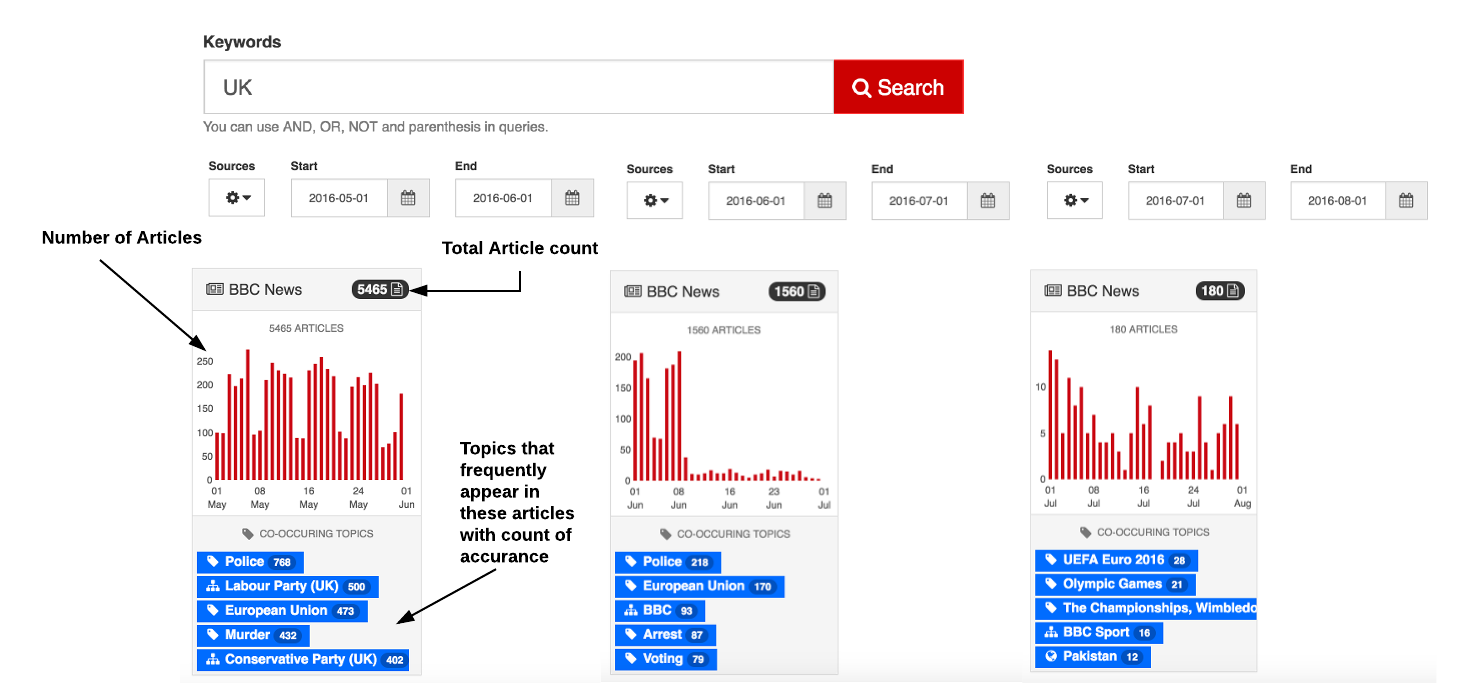
\includegraphics[width=\textwidth]{figures/BBC_wat.png}
\caption{Example of the topic evolution on BBC News: Who's talking about what ?}
\label{fig:bbc_wat}
\end{figure}

The other challenge is to apply author-topic (AT) model for the news collection which simultaneously model the content of the document and also the interest of the authors. The advantage of AT model is that besides representing each news with a mixture of topics, the \textit{author} is also modeled by determining the mixture weights for different topics for a single news, each \textit{author} is associated with a multinomial distribution over topics. This generative model perfectly fits in the corporus of BBC news, since for BBC news there is a virtual \textit{author} for each of the news, which is its category, as shown in ~\ref{tab:news_category}. For news in different categories their prose style will differ in the aspects of vocabulary use,  sentence structure, as well as the way in which stories present the information in terms of relative importance, tone, and intended audience. 

So the BBC news can be assumed to be generated in the following way, as shown in Figure~\ref{fig:author_diagram}.

\begin{enumerate}
   \item For each topic $k \in [1,K]$
   \begin{enumerate}
     \item Draw a multinomial $\vec{\phi_k}$ from a Dirichlet prior $\vec{\beta}$
    \end{enumerate}
   \item For each author $a \in [1,A]$
   \begin{enumerate}
     \item Draw a multinomial $\vec{\theta_a}$ from a Dirichlet prior $\vec{\alpha}$
    \end{enumerate}
    \item For each news $m \in [1,M]$
   \begin{enumerate}
     \item For each word $n \in [1,N_m]$ in document $m$
     \begin{enumerate}
            \item Draw an author $x_{m,n}$ uniformly from the group of authors $a_M$
            \item Draw a topic assignment $z_{m,n}$ from per-author multinomila distribution over topic $\vec{\theta_{x_{m,n}}}$
            \item Draw a word $w_{m,n}$ from multinomial $\vec{\phi_{z_{m,n}}}$
    \end{enumerate}
    \end{enumerate}
        
\end{enumerate}

In the above process the posterior distribution of topics are dependent on the information form the authors as well as the text of the news. The parameterization of the AT model can be seen in Section ~\ref{Author-Topic model}

\begin{figure}[h]
\centering
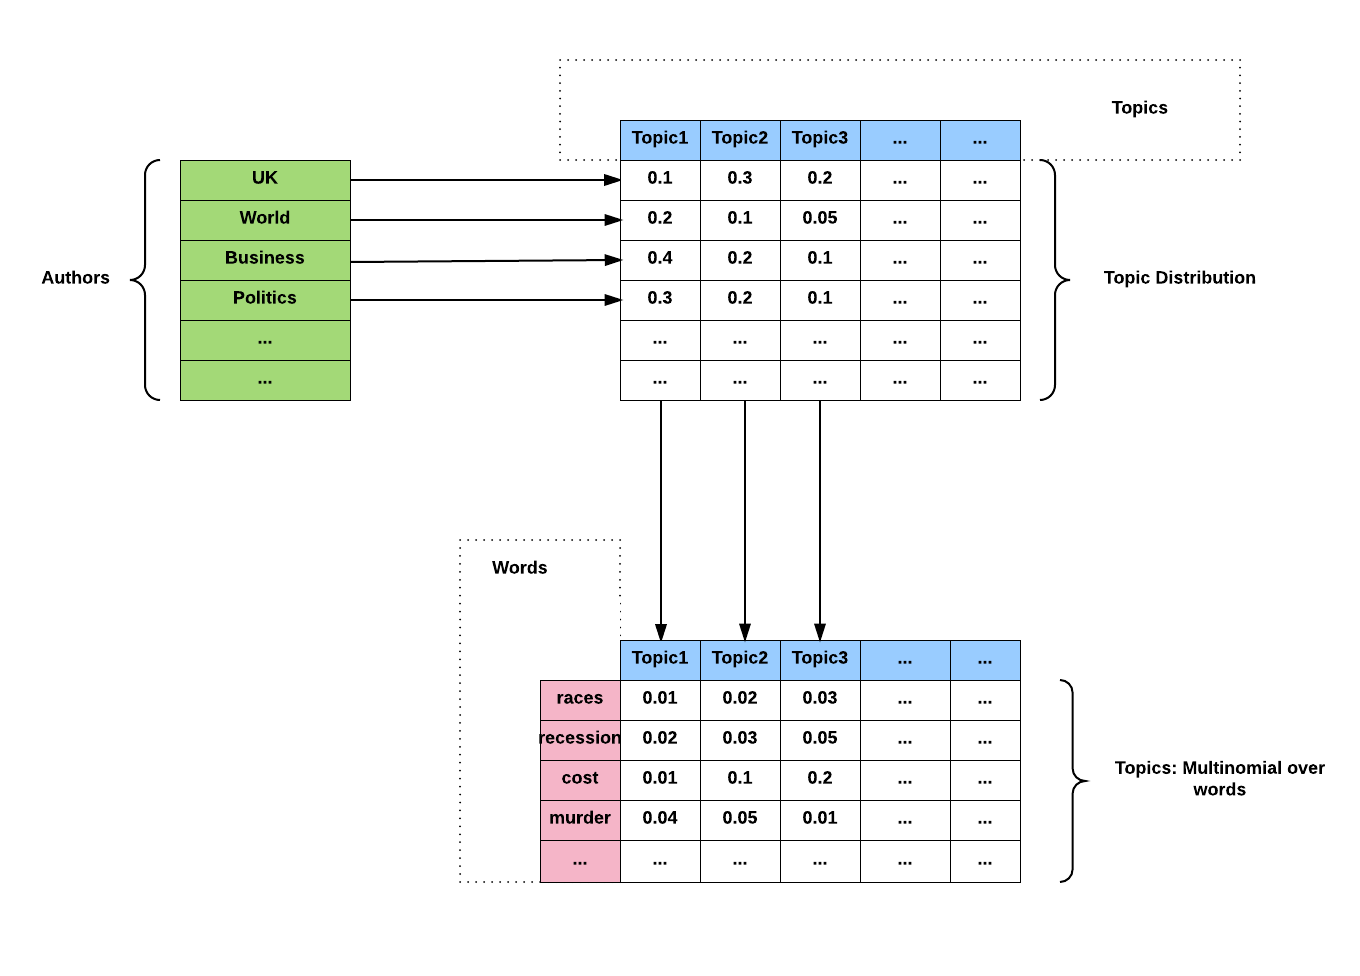
\includegraphics[width=\textwidth]{figures/author_diagram.png}
\caption{Illustration of generative models for BBC news document}
\label{fig:author_diagram}
\end{figure}


Therefore in order to encompass the extra-feature of the news, namely its category, in our model, the AT model is used as the basis of our dynamic model to overcome the above two challenges. Here we define the concepts of \textbf{\textit{topic}} and \textbf{\textit{author}} as follows: 
\begin{itemize}
  \item A \textbf{\textit{topic}} is a subject discussed in one or more news. Examples of topics include events such as "UK referendum" entities such as "David Cameron " and long-standing subjects such as "UK Politics". Each topic is assumed to be represented by a multinomial distribution of words.
  \item An \textbf{\textit{author}} is a category of BBC news which groups topics belonging to a common subject
  area together. Examples of authors include BBC news categories of "UK", "World", "Eduction", "Health", etc, as listed in ~\ref{tab:news_category}
  \end{itemize}
The model we propose here is Dynamic Author-Topic (DAT) model which draws upon the strength of author-topic model and dynamic topic model. Considering the temporal nature of news we assume the topic distributions of news will evolve over time frames (a day, a week or a month), and the inferred topic distribution in the past news documents will become the evidence of those for the current new. In each time frame, we assume the news are generated based on author-topic model. Information about which topics are associated to which author and the representation of the content of each news document in terms of topics are derived and used for the next time frame. The details are discussed in the following sections.

\section{Task Description}\label{taskdescription}
The task that is addressed in this thesis can fall in the following 3 aspects

\begin{itemize}
  \item \textbf{Tagging}: Based on the content and time of the news we are able to automatically tag the news with an author (category)
  \item \textbf{Summarization}: Based on the author-topic distribution we are able to what topics are most discussed in one type of news
  \item \textbf{Dynamics}: We are able to monitor the changes of event of interest for the news over time
\end{itemize}

The input of our model will be the BBC news text in a range of time,

\begin{figure}[h]
\centering
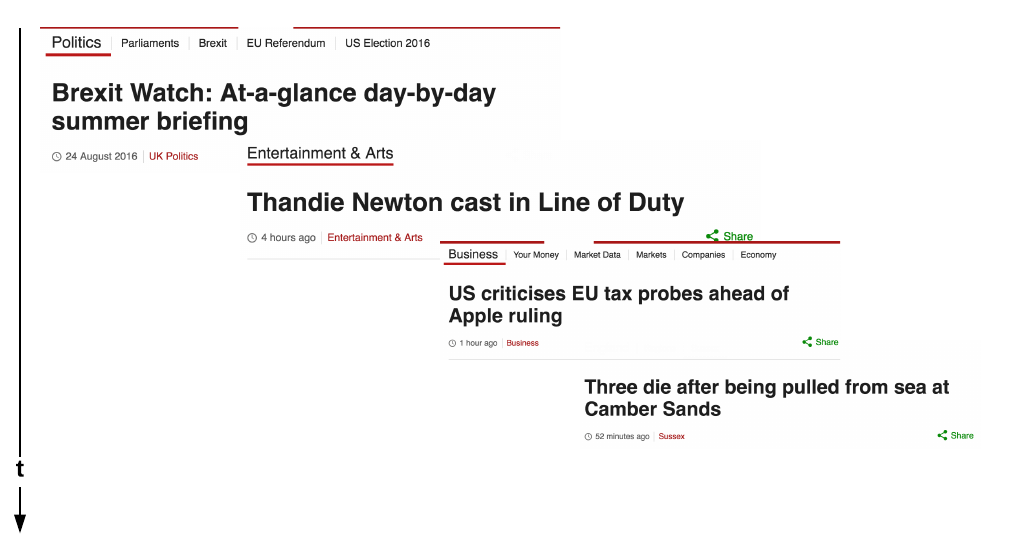
\includegraphics[width=\textwidth]{figures/input.png}
\caption{Input: BBC News over time}
\label{fig:input}
\end{figure}

The output will satisfies the above 3 aspects, as shown in Figure ~\ref{fig:output}
\begin{figure}[h]
\centering
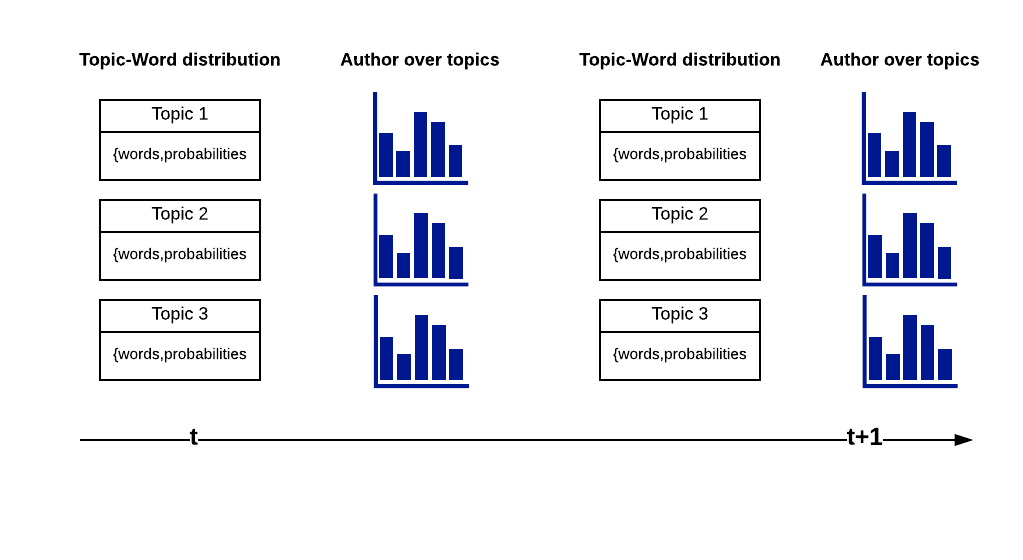
\includegraphics[width=\textwidth]{figures/output.png}
\caption{Output: Temporal evolution of topics and authors’ proportion over the topics }
\label{fig:output}
\end{figure}



Mathematically, the author-topic and topic-words distribution are changing dynamically with news stream in, our dynamic model is essentially a function $f$ that satisfies:
\begin{equation}
\label{eq:task}
\mathbf{m}_{\le t}=\{\ldots, \mathbf{m}_{t-2}', \mathbf{m}_{t-1}', \mathbf{m}_t'\}
\stackrel{f}{\longrightarrow} \boldsymbol W'_{\boldsymbol a,\boldsymbol k}_{\le t}=\{\{\mathbf{w}_1', \mathbf{w}_2', \ldots, \mathbf{w}_K'\},\{\mathbf{w}_1', \mathbf{w}_2', \ldots, \mathbf{w}_A'\}\}
\end{equation}

in which $\mathbf{m}_{\le t}$ represents news stream with $\mathbf{m}_t'$ being the most recent \textit{set} news, arring at time $t$, with our dynamic model it results in  $\boldsymbol W'_{\boldsymbol a,\boldsymbol k}$ is the resulting set of 3-tuple, $\{w,a,k\}$, which represents word $w$ and the author $a$ and topic $k$ assigned to it, with $\mathbf{w}_k'$ being the words set associated with topic $k$,  with $\mathbf{w}_a'$ being the words set associated with author $a$-th.

$\mathbf{m}'_t$ comprises a the stream of news at time $t$, with each news $m$ being represented by a sequence of words appearing in $m$, coming from the vocabulary $\boldsymbol w$. % and $t$ is the creation time of the document $d$.
%$\mathbf{d}'_t$ comprises a set of short text documents, with each document being represented by a tuple $\langle \mathbf{w}_d, t \rangle$ where $\mathbf{w}_d$ is a sequence of words appearing in document $d$, coming from a vocabulary $\mathbf{V}=\{ v_1, v_2, \ldots, v_V\}$, and $t$ is the creation time of the document $d$. 

Based on $\boldsymbol W'_{\boldsymbol a,\boldsymbol k}$ we are able to calculate the author-topic and topic-word distribution to see the topic evolution over time.
Table ~\ref{tab:notation-des} summarises the main notations that we have used in our dynamic author-topic model.
\begin{table}[h]
\center
\vspace{-1pt}
\caption{Notation used in the Dynamic Author-topic model}
\label{tab:notation-des}
\small
\begin{tabular}{ll}
Symbol & Description\\
\hline

$\bs{K}$ & Number of latent topics\\
$\bs{M}$ & Number of news\\
$\bs{A}$ & Number of unique authors\\
$\bs{A_m}$ & Number of authors in document $m$\\
$\bs{V}$ & Number of unique word tokens in the whole news corpus\\
$T$ & Number of time frames  \\
$N_{\text{m}}$ & Number of word tokens in news m\\
$k$ & Topic index,  $k \in [1,\bs{K]$ \\
$m$ & News index,  $m \in [1,M]$ \\
$a$ & Author index,  $a \in [1,\bs{A}]$ \\
$t$ & Time frame index, $t \in [1,T]$\\
$n$ & Word index in document $m$,  $n \in [1,N_{\text{m}}]$ \\
$v$ & Word index in the whole news document corpus,  $v \in [1,V]$ \\
$\boldsymbol a$ & Set of all authors \\
$\boldsymbol k$ & Set of all topics \\
$\boldsymbol m$ & Set of all news \\
$\boldsymbol m'_t$ & Set of news at time t\\
$\boldsymbol w$ & Words set for all news \\
$\boldsymbol w'_{a}$ & Words set comprising words associated with author $a$ \\
$\boldsymbol w'_{k}$ & Words set comprising words associated with topic $k$ \\
$\boldsymbol W'_{\boldsymbol a,\boldsymbol k}$ & The set of 3-tuple, $\{w,a,k\}$, which represents word $w$ and the author $a$ and topic $k$ assigned to it \\
$\boldsymbol w_m$ & Words set for news $m$ \\
$\alpha_{t}$ & Parameter of topic Dirichlet prior to $\theta$ at time $t$ \\
$\beta{t}$ & Parameter of word Dirichlet prior to $\phi$ at time $t$ \\
$a_m$ & Authors in news m,  $a_m \in [1,\bs{A]$ \\
$\theta_{a,t}$ & Dynamic multinomial distribution of topics specified to author $a$ at time $t$ \\
$\phi_{k,t}$ & Dynamic multinomial distribution of words specified to topic $k$ at time $t$ \\
$x_{m,n}$ & Author associated to $w_{m,n}$ \\
$z_{m,n}$ & Topic associated to $w_{m,n}$ \\
$w_{m,n}$ & $n_{th}$ word in doc $n$ \\



\end{tabular}
\end{table}

\section{Dynamic Author-Topic Model}
To meet the requirements discussed in ~\ref{taskdescription}, so that the event interests of the news can be  














The parameterization of the proposed dynamic author-topic model is as follows:
\begin{eqnarray*} \label{eq:dat}
\boldsymbol{\Theta}_{a,t} | \boldsymbol{\alpha_{a,t}}
\boldsymbol{\Theta}_{a,t-1}
& \sim & \text{Dirichlet}{\boldsymbol{\alpha_{a,t}}
\boldsymbol{\Theta}_{a,t-1}}\\
\boldsymbol{\Phi_{k,t}} | \boldsymbol{\beta_{k,t}}\boldsymbol{\Phi_{k,t-1}} & \sim & \text{Dirichlet}(\boldsymbol{\beta_{k,t}}\boldsymbol{\Phi_{k,t-1}})\\
z_{m,n} | \boldsymbol{\Theta_{x_{m,n},t}} & \sim & \text{Multinomial}(\boldsymbol{\Theta_{x_{m,n},t}})\\
w_{m,n} | \boldsymbol{\Phi_{z_{m,n},t}} & \sim & \text{Multinomial}(\boldsymbol{\Phi_{z_{m,n},t}})\\
x_{m,n} | {A_{m}} & \sim & \text{Multinomial}(1/A_m)\\

\end{eqnarray*}

\begin{figure}[h]
\centering
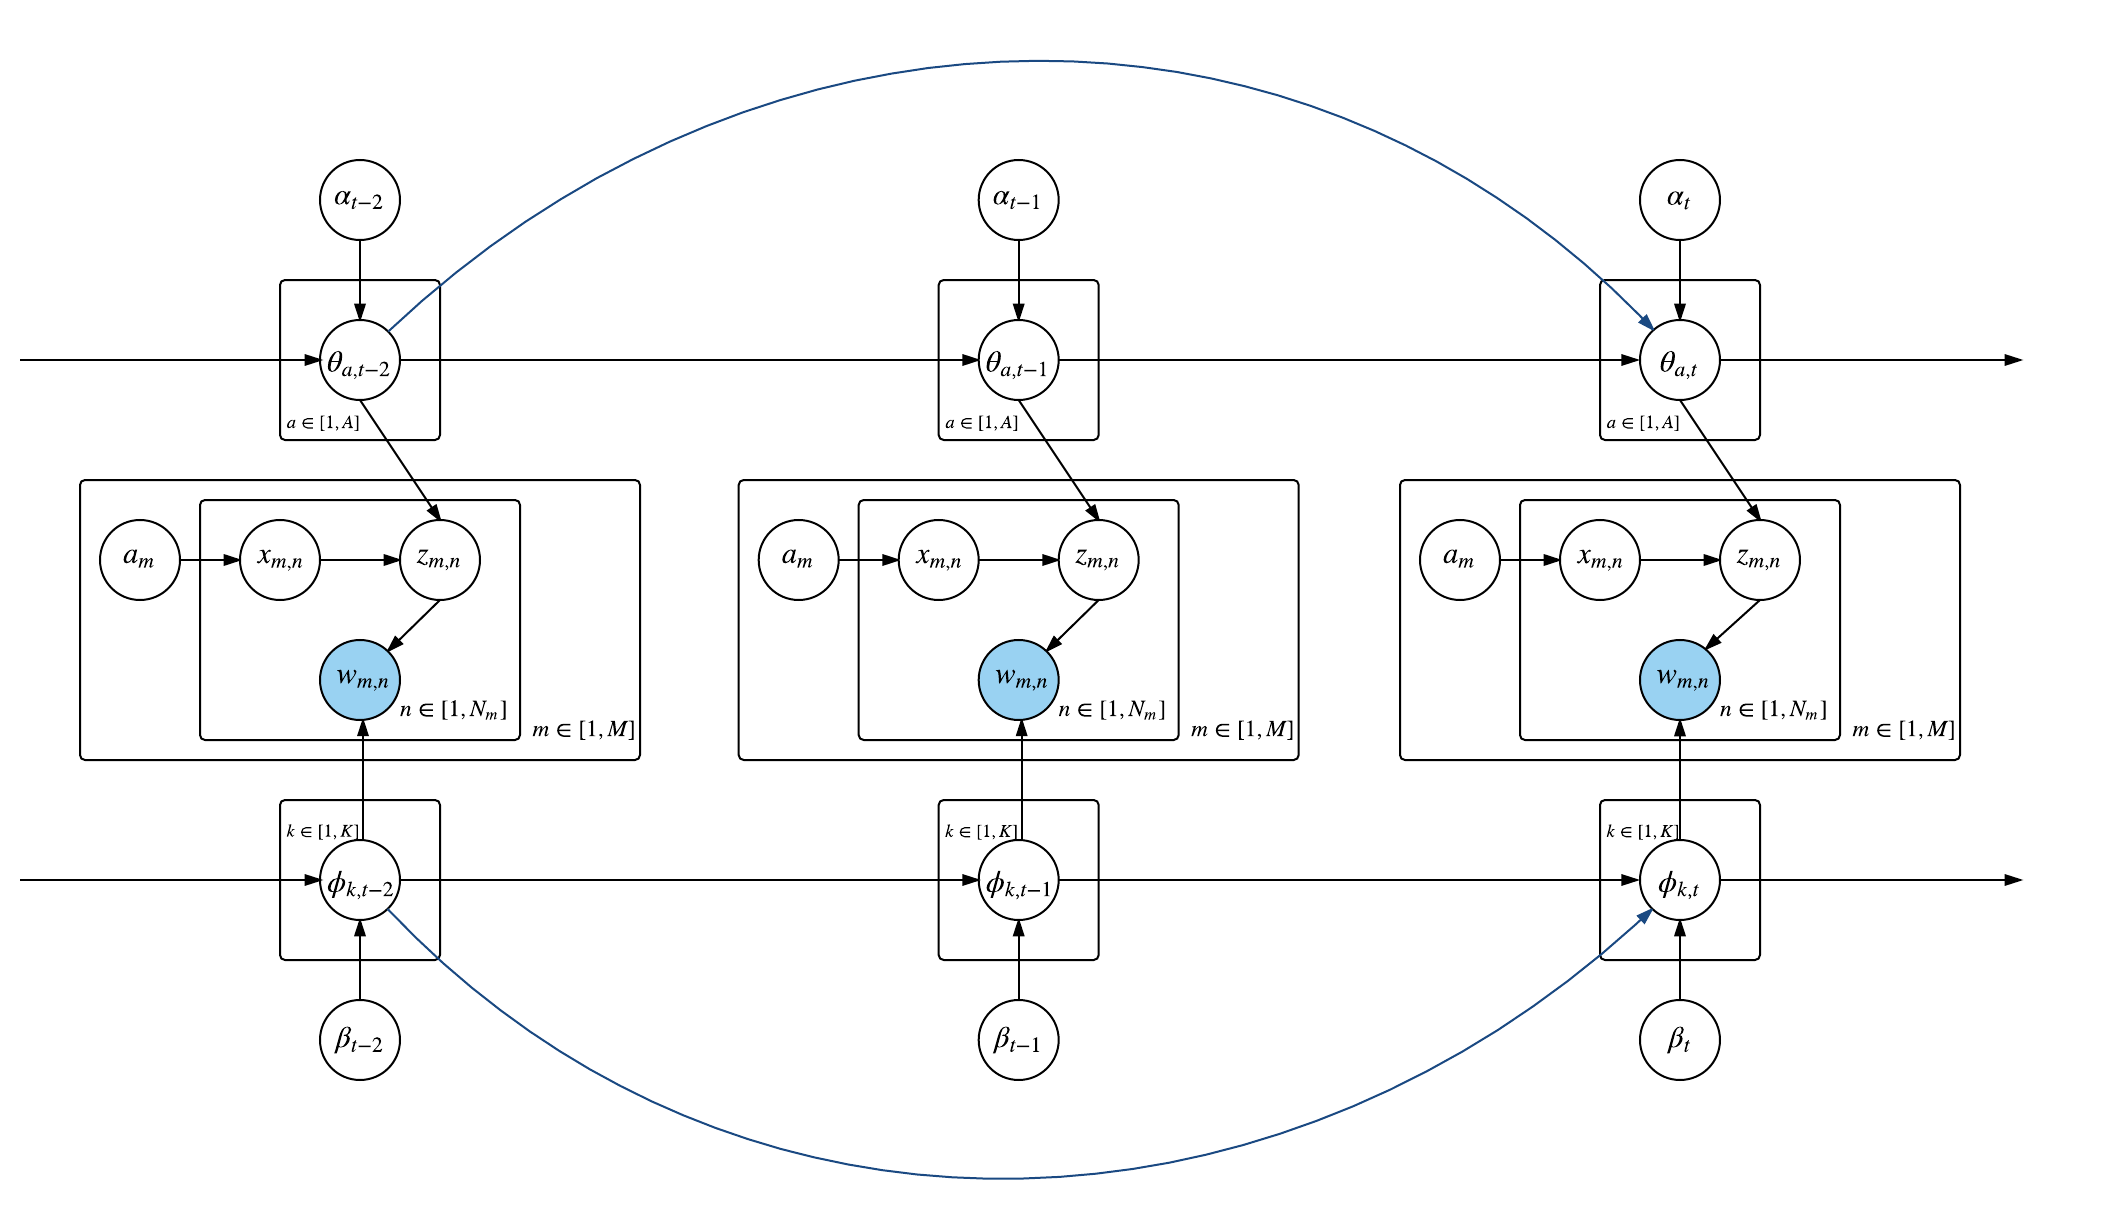
\includegraphics[width=\textwidth]{figures/ATOT_Graphic.png}
\caption{Graphical representation of our dynamic author-topic model, DAT model. Note that short term dependency DAT model excludes the two blue curved lines , the long term dependency DAT model includes the two lines.}
\label{fig:atot}
\end{figure}









\section{Model Inference}

Similar to LDA model, based on the algorithm proposed by \cite{blei2003latent} to calculate the approximate maximum likelihood estimates for $\boldsymbol{\phi}$ as well as the hyperparameter of the prior $\boldsymbol{\theta}$, the Markov Chain Monte Carlo (MCMC) is used for inference, MCMC is an approach to obtain the sample from the complicated probability distributions, to allow a Markov chain to converge to a targeted distribution and the drawing the samples from the Markov chain \cite{gilks1996introducing}. Gibbs Sampling is used here for the inference in which the next state is arrived by sampling all variables from their distribution sequentially when conditioned on the current values of all other variables and the data.
in the above Gibbs sampling procedure, we need to calculate the conditional distribution first, which is
\begin{equation}
P({z}_{m, n, t},{x}_{m, n, t}| \mathbf{w}_t,\mathbf{z}_{\neg(m, n, t)}, \mathbf{x}_{\neg(m, n, t)},\mathbf{a_t},\alpha_t, \beta_t,\boldsymbol{\Phi}_{t-1}, \boldsymbol{\Theta}_{t-1})
\label{eq:conditional}
\end{equation}
where $\mathbf{z}_{\neg(m, n, t)}, \mathbf{x}_{\neg(m, n, t)}$ represents the topic, author assignments for all the word tokens in the news corpus except for $w_{m,n}$. We can begin with the joint distribution,
\begin{equation}
P(\mathbf{w}_t, \mathbf{z}_t ,\mathbf{x}_t| \alpha_t, \beta_t,\mathbf{a}, \boldsymbol{\Phi}_{t-1}, \boldsymbol{\Theta}_{t-1})
\end{equation}
so that we can take advantage of the conjugate priors to simplify the integrals. The symbols used here are all defined in Table~\ref{tab:notation-des}. The whole process of Gibbs sampling derivation for our dynamic author-topic model is listed as follows.
\begin{align*}
\multicolumn{2} =   &  \math{P}({z}_{m, n, t},{x}_{m, n, t}| \mathbf{w}_t,\mathbf{z}_{\neg(m, n, t)}, \mathbf{x}_{\neg(m, n, t)},\mathbf{a_t},\alpha_t, \beta_t,\boldsymbol{\Phi}_{t-1}, \boldsymbol{\Theta}_{t-1})
\displaybreak[3]\\
\propto & \quad P(\mathbf{w}_t, \mathbf{z}_t ,\mathbf{x}_t| \alpha_t, \beta_t,\mathbf{a_t}, \boldsymbol{\Phi}_{t-1}, \boldsymbol{\Theta}_{t-1}) \displaybreak[3]\\
& \hspace{-0.1in}\text{based on the graphical model in Figure ~\ref{fig:atot}, and integrate on $\boldsymbol{\Phi}$ and $\boldsymbol{\Theta}$ it becomes}\displaybreak[3]\\
= & \quad  P(\mathbf{w}_t | \mathbf{z}_t, \mathbf{\beta}_t,\boldsymbol{\Phi}_{t-1})\times P(\mathbf{z}_t | \boldsymbol{\Theta}_{t-1}, \alpha_t, \mathbf{x}_t) \times P(\mathbf{x}_t | \mathbf{a}_t) \displaybreak[3]\\
= & \quad \int P(\mathbf{w}_t | \mathbf{z}_t, \boldsymbol{\Phi}_t) P(\boldsymbol{\Phi}_t | \boldsymbol{\Phi}_{t-1}, \beta_t) d\boldsymbol{\Phi}_t \int P(\mathbf{z}_t | \mathbf{x}_t, \boldsymbol{\Theta}_t) P(\boldsymbol{\Theta}_t | \boldsymbol{\Theta}_{t-1}, \alpha_t) d\boldsymbol{\Theta}_t \displaybreak[3]\\
&  \times P(\mathbf{x}_t | \mathbf{a}_t)\displaybreak[3]\\
& \hspace{-0.1in}\text{we then rewrite the probabilistic distribution from the way of vector to that of scalar, }\\
& \hspace{-0.1in}\text{for example, $P(\mathbf{w}_t | \mathbf{z}_t, \boldsymbol{\Phi}_t)$ can become the the product of $P({w}_{m, n, t} | \phi_{t, z_{m,n}})$      across the}\\
& \hspace{-0.1in}\text{whole corpus, it becomes,}\displaybreak[3]\\
= & \quad \int \prod_{m=1}^{M} \prod_{n=1}^{N_m} P({w}_{m, n, t} | \phi_{t, z_{m,n}}) \prod_{k=1}^K P(\phi_{t, k} | \phi_{t-1,k}, \beta_t) d\Phi_t \displaybreak[3]\\
&  \times \int \prod_{m=1}^{M} \prod_{n=1}^{N_m} P({z}_{m, n, t} | {\theta}_{x_{m,n}},t) \prod_{a=1}^{A}P(\theta_{a,t}|\theta_{a,t-1},\alpha_t) d\Theta_t \displaybreak[3]\\
&  \times \prod_{m=1}^{M} \prod_{n=1}^{N} P({x}_{m, n, t} | {a}_{m,t}) \displaybreak[3]\\
& \hspace{-0.1in}\text{since extract the word $w_{m,n}$ from topic $z_{n,n}$ exactly follow the distribution of $\phi_{z_{m,n}}$, and }\displaybreak[3]\\
& \hspace{-0.1in}\text{also extract topic $z_{m,n}$ from the author $x_{m,n}$ similarly follow the distribution of $\theta_{x_{m,n}}$, so, }\displaybreak[3]\\
= & \quad \int \prod_{k=1}^K \prod_{v=1}^V \phi_{t, v, k}^{n_{(t, v,k)}} \prod_{k=1}^K P(\phi_{t, k} | \phi_{t-1, k}, \beta_t) d\Phi_t \displaybreak[3]\\
&  \times \int \prod_{a=1}^A \prod_{k=1}^K \theta_{t, a, k}^{n_{(t, a,k)}} \prod_{a=1}^A P(\theta_{a,t}|\theta_{a,t-1},\alpha_t) d\Theta_t \times \left(\frac{1}{\prod_{m=1}^M A_m^{N_m}} \right) \displaybreak[3]\\
%
& \hspace{-0.1in}\text{based on the posterior of  Dirichlet distribution \cite{ferguson1973bayesian} }\displaybreak[3]\\
= & \quad \int \prod_{k=1}^K \prod_{v=1}^V \phi_{t,v,k}^{n_{(t,v,k)}} \prod_{k=1}^K \left( \frac{\mathrm{\Gamma} (\sum_{v=1}^V \beta_{(t, k, v)} {\phi_{t-1}})}{\prod_{v=1}^V \mathrm{\Gamma}(\beta_{(t, k, v)} {\phi_{t-1}})} \prod_{v=1}^V \phi_{t, k, v}^{\left(\beta_{(t, k, v)} {\phi_{t-1}} \right) -1} \right) d\Phi_t \displaybreak[3]\\
%
&  \times \int \prod_{a=1}^A \prod_{k=1}^K \theta_{t, a, k}^{n_{(t, a,k)}} \prod_{a=1}^A \left( \frac{\mathrm{\Gamma}(\sum_{k=1}^k \alpha_{(t, k)} \theta_{t-1, k})}{\prod_{k=1}^K \mathrm{\Gamma} (\alpha_{(t, k)} \theta_{t-1, k})} \prod_{k=1}^K \Theta_{t, k}^{\left(\alpha_{(t, k)} {\Theta_{t-1,k}} \right) -1}  \right)  d\Theta_t \displaybreak[3]\\
%
&  \times \left(\frac{1}{\prod_{m=1}^M A_m^{N_m}} \right) \displaybreak[3]\\
%
%
%= & \prod_{z=1}^Z \frac{\mathrm{\Gamma} (\sum_{v=1}^V \beta_{t, z, v} \abbrev{\phi})}{\prod_{v=1}^V \mathrm{\Gamma}(\beta_{t, z, v} \abbrev{\phi})} \int \prod_{z=1}^Z \prod_{v=1}^V \phi_{t, z, v}^{n_{t, z, v}} \prod_{z=1}^Z \prod_{v=1}^V \phi_{t, z, v}^{\beta_{t, z, v} \abbrev{\phi} -1} d\Phi_t \displaybreak[3]\\
%& \times \frac{\mathrm{\Gamma}(\sum_{z=1}^Z \alpha_{t, z} \theta_{t-1, z})}{\prod_{z=1}^Z \mathrm{\Gamma} (\alpha_{t, z} \theta_{t-1, z})} \int \prod_{z=1}^Z \theta_{t, z}^{m_{t, z}}  \prod_{z=1}^Z \theta_{t, z}^{\alpha_{t, z} \theta_{t-1, z} -1} d\Theta_t \displaybreak[3]\\
%
& \hspace{-0.1in}\text{since for different topics , based on d-separation \cite{geiger2013d} their topic-word distribution  }\displaybreak[3]\\
& \hspace{-0.1in}\text{can be regarded as independent from each other, which is the same for author-topic   }\displaybreak[3]\\
& \hspace{-0.1in}\text{distributions, so that the integration of products can be rewritten as product of integrations,}\displaybreak[3]\\
= & \quad \prod_{k=1}^K \frac{\mathrm{\Gamma} (\sum_{v=1}^V \beta_{(t, k, v)} {\phi_{t-1}})}{\prod_{v=1}^V \mathrm{\Gamma}(\beta_{(t, k, v)} {\phi_{t-1}})} \prod_{k=1}^K \int \prod_{v=1}^V \phi_{t, v,k}^{n_{t, v,k}+\beta_{t, k,v} {\phi_{t-1}} -1} d\Phi_t \displaybreak[3]\\
& \times \prod_{a=1}^A \frac{\mathrm{\Gamma}(\sum_{k=1}^K \alpha_{(t, k)} \theta_{t-1, k})}{\prod_{k=1}^K \mathrm{\Gamma} (\alpha_{(t, k)} \theta_{(t-1, k)})} \prod_{a=1}^A \int \prod_{k=1}^K \theta_{t, k}^{n_{t,a,k}+\alpha_{t, k} \theta_{t-1, k} -1} d\Theta_t \displaybreak[3]\\
& \times \left(\frac{1}{\prod_{m=1}^M A_m^{N_m}} \right) \displaybreak[3]\\
& \hspace{-0.1in}\text{according to Euler integral \cite{jeffrey2008handbook},}\displaybreak[3]\\
= & \quad \prod_{k=1}^K \frac{\mathrm{\Gamma} (\sum_{v=1}^V \beta_{t, k, v} {\phi_{t-1}})}{\prod_{v=1}^V \mathrm{\Gamma}(\beta_{t, k, v} {\phi_{t-1}})} \prod_{k=1}^K \frac{\prod_{v=1}^V \mathrm{\Gamma} (n_{t,v,k} + \beta_{t, k, v} {\phi_{t-1}})}{\mathrm{\Gamma} (\sum_{v=1}^V n_{t,v,k} + \beta_{t, k, v} {\phi_{t-1}})} \displaybreak[3]\\
&  \times \prod_{a=1}^A \frac{\mathrm{\Gamma}(\sum_{k=1}^K \alpha_{t, k} \theta_{t-1, k})}{\prod_{k=1}^K \mathrm{\Gamma} (\alpha_{t, k} \theta_{t-1, k})}  \prod_{a=1}^A \frac{\prod_{k=1}^K \mathrm{\Gamma} (n_{t,a,k} + \alpha_{t, k} \theta_{t-1, k})}{\mathrm{\Gamma} (\sum_{k=1}^K n_{t,a, k} + \alpha_{t, k} \theta_{t-1, k})} \displaybreak[3]\\
& \times   \left(\frac{1}{\prod_{m=1}^M A_m^{N_m}} \right) \displaybreak[3]\\
%
\end{align*}
where $n_{t,a,k} = n_{a,t}^(k) $ representing the number of times the author $a$ is assigned to topic $k$, at time $t$, and $n_{t,v,k}$ representing the number of times word token $v$ is assigned to topic $k$, at time $t$.
Applying the chain rule, we can obtain the conditional probability,

\begin{align*}
\multicolumn{2} =   &  \math{P}({z}_{m, n, t},{x}_{m, n, t}| \mathbf{w}_t,\mathbf{z}_{\neg(m, n, t)}, \mathbf{x}_{\neg(m, n, t)},\mathbf{a_t},\alpha_t, \beta_t,\boldsymbol{\Phi}_{t-1}, \boldsymbol{\Theta}_{t-1})
\displaybreak[3]\\
= & \quad \frac{\math{P}({w}_{m, n,t},{z}_{m, n, t},{x}_{m, n, t}| \mathbf{w}_{\neg(m, n, t)},\mathbf{z}_{\neg(m, n, t)}, \mathbf{x}_{\neg(m, n, t)},\mathbf{a_t},\alpha_t, \beta_t,\boldsymbol{\Phi}_{t-1}, \boldsymbol{\Theta}_{t-1})}{\math{P}({w}_{m, n, t}| \mathbf{w}_{\neg(m, n, t)},\mathbf{z}_{\neg(m, n, t)}, \mathbf{x}_{\neg(m, n, t)},\mathbf{a_t},\alpha_t, \beta_t,\boldsymbol{\Phi}_{t-1}, \boldsymbol{\Theta}_{t-1})}
\displaybreak[3]\\
= & \quad \frac{P(\mathbf{w}_t, \mathbf{z}_t,\mathbf{x}_t |  \alpha_t, \beta_t, \boldsymbol{\Phi}_{t-1}, \boldsymbol{\Theta}_{t-1})}{P(\mathbf{w}_{t}, \mathbf{z}_{t,\neg(m,n)},\mathbf{x}_{t,\neg(m,n)} | \alpha_t, \beta_t,a, \boldsymbol{\Phi}_{t-1}, \boldsymbol{\Theta}_{t})} \displaybreak[3]\\
%
= & \quad \frac{P(\mathbf{w}_t, \mathbf{z}_t,\mathbf{x}_t |  \alpha_t, \beta_t, \boldsymbol{\Phi}_{t-1}, \boldsymbol{\Theta}_{t-1})}{P(\mathbf{w}_{t,\neg(m,n)}, \mathbf{z}_{t,\neg(m,n)},\mathbf{x}_{t,\neg(m,n)} | \alpha_t, \beta_t,a, \boldsymbol{\Phi}_{t-1}, \boldsymbol{\Theta}_{t})P(w_{m,n,t} |  \alpha_t, \beta_t, \boldsymbol{\Phi}_{t-1}, \boldsymbol{\Theta}_{t-1})} \displaybreak[3]\\
\propto & \quad \frac{P(\mathbf{w}_t, \mathbf{z}_t,\mathbf{x}_t |  \alpha_t, \beta_t, \boldsymbol{\Phi}_{t-1}, \boldsymbol{\Theta}_{t-1})}{P(\mathbf{w}_{t,\neg(m,n)}, \mathbf{z}_{t,\neg(m,n)},\mathbf{x}_{t,\neg(m,n)} | \alpha_t, \beta_t,a, \boldsymbol{\Phi}_{t-1}, \boldsymbol{\Theta}_{t})} \displaybreak[3]\\
\propto & \quad \prod_{k=1}^K \frac{\mathrm{\Gamma} (\sum_{v=1}^V \beta_{t, k, v} {\phi_{t-1}})}{\prod_{v=1}^V \mathrm{\Gamma}(\beta_{t, k, v} {\phi_{t-1}})} \prod_{k=1}^K \frac{\prod_{v=1}^V \mathrm{\Gamma} (n_{t,v,k} + \beta_{t, k, v} {\phi_{t-1}})}{\mathrm{\Gamma} (\sum_{v=1}^V n_{t,v,k} + \beta_{t, k, v} {\phi_{t-1}})} \displaybreak[3]\\
&  \times \prod_{a=1}^A \frac{\mathrm{\Gamma}(\sum_{k=1}^K \alpha_{t, k} \theta_{t-1, k})}{\prod_{k=1}^K \mathrm{\Gamma} (\alpha_{t, k} \theta_{t-1, k})}  \prod_{a=1}^A \frac{\prod_{k=1}^K \mathrm{\Gamma} (n_{t,a,k} + \alpha_{t, k} \theta_{t-1, k})}{\mathrm{\Gamma} (\sum_{k=1}^K n_{t,a, k} + \alpha_{t, k} \theta_{t-1, k})} \displaybreak[3]\\
& \hspace{-0.1in}\text{applying $\mathrm{\Gamma}(x)=(x-1)\mathrm{\Gamma}(x-1)$ and $\mathrm{\Gamma}(x+m)=\prod_{i=1}^m (x+i-1)\mathrm{\Gamma}(x)$, and considering } \displaybreak[3]\\
& \hspace{-0.1in}\text{that author $a$ is associated with its own topic $z$, the above becomes} \displaybreak[3]\\
\propto & \quad  \left(\frac{n_{t,v,k}+\beta_{t,k,v}\phi_{t-1}-1}{\sum_{v=1}^V \left(n_{t,v,k}+\beta_{t,v,k}\phi_{t-1} \right)-1 } \right) \times   \left(\frac{n_{t,a,k}+\alpha_{t,k} \Theta_{t-1}-1}{\sum_{k=1}^K \left(n_{t,a,k}+\alpha_{t,k}\theta_{t-1} \right)-1 } \right)
\displaybreak[3]\\
\end{align*}

If we manipulate the above formula to turn the above update equations for the topic and author of each token into separated updated ones, which can obtain the following update rules which are suitable for random or systematic scan updates, 
\begin{itemize}
  \item For the topic:
  \begin{align*}
\multicolumn{2} =   &  \math{P}({z}_{m, n, t}| \mathbf{w}_t,\mathbf{z}_{\neg(m, n, t)},\mathbf{x}_t, \mathbf{a_t},\alpha_t, \beta_t,\boldsymbol{\Phi}_{t-1}, \boldsymbol{\Theta}_{t-1})
\displaybreak[3]\\
= & \quad \frac{\math{P}({w}_{m, n, t},{z}_{m, n, t}| \mathbf{w}_{\neg(m, n, t)},\mathbf{z}_{\neg(m, n, t)},\mathbf{x}_t, \mathbf{a_t},\alpha_t, \beta_t,\boldsymbol{\Phi}_{t-1}, \boldsymbol{\Theta}_{t-1})}{\math{P}({w}_{m, n, t}| \mathbf{w}_{\neg(m, n, t)},\mathbf{z}_{\neg(m, n, t)},\mathbf{x}_t, \mathbf{a_t},\alpha_t, \beta_t,\boldsymbol{\Phi}_{t-1}, \boldsymbol{\Theta}_{t-1})}
\displaybreak[3]\\
= & \quad \frac{P(\mathbf{w}_t, \mathbf{z}_t | \mathbf{x}_t, \alpha_t, \beta_t, \boldsymbol{\Phi}_{t-1}, \boldsymbol{\Theta}_{t-1})}{P(\mathbf{w}_{t}, \mathbf{z}_{t,\neg(m,n)} |\mathbf{x}_t, \alpha_t, \beta_t,\mathbf{a_t}, \boldsymbol{\Phi}_{t-1}, \boldsymbol{\Theta}_{t})} \displaybreak[3]\\
= & \quad \frac{P(\mathbf{w}_t, \mathbf{z}_t | \mathbf{x}_t, \alpha_t, \beta_t, \boldsymbol{\Phi}_{t-1}, \boldsymbol{\Theta}_{t-1})}{P(\mathbf{w}_{t,\neg(m,n)}, \mathbf{z}_{t,\neg(m,n)} | \mathbf{x}_{t},\alpha_t, \beta_t,\mathbf{a_t}, \boldsymbol{\Phi}_{t-1}, \boldsymbol{\Theta}_{t})P(w_{m,n} | \mathbf{x}_{t}, \alpha_t, \beta_t, \boldsymbol{\Phi}_{t-1}, \boldsymbol{\Theta}_{t-1})} \displaybreak[3]\\
\propto & \quad \frac{P(\mathbf{w}_t, \mathbf{z}_t | \mathbf{x}_t, \alpha_t, \beta_t, \boldsymbol{\Phi}_{t-1}, \boldsymbol{\Theta}_{t-1})}{P(\mathbf{w}_{t,\neg(m,n)}, \mathbf{z}_{t,\neg(m,n)} | \mathbf{x}_{t},\alpha_t, \beta_t,\mathbf{a_t}, \boldsymbol{\Phi}_{t-1}, \boldsymbol{\Theta}_{t})} \displaybreak[3]\\
%
\propto & \quad \prod_{k=1}^K \frac{\mathrm{\Gamma} (\sum_{v=1}^V \beta_{t, k, v} {\phi_{t-1}})}{\prod_{v=1}^V \mathrm{\Gamma}(\beta_{t, k, v} {\phi_{t-1}})} \prod_{k=1}^K \frac{\prod_{v=1}^V \mathrm{\Gamma} (n_{t,v,k} + \beta_{t, k, v} {\phi_{t-1}})}{\mathrm{\Gamma} (\sum_{v=1}^V n_{t,v,k} + \beta_{t, k, v} {\phi_{t-1}})} \displaybreak[3]\\
&  \times \prod_{a=1}^A \frac{\mathrm{\Gamma}(\sum_{k=1}^K \alpha_{t, k} \theta_{t-1, k})}{\prod_{k=1}^K \mathrm{\Gamma} (\alpha_{t, k} \theta_{t-1, k})}  \prod_{a=1}^A \frac{\prod_{k=1}^K \mathrm{\Gamma} (n_{t,a,k} + \alpha_{t, k} \theta_{t-1, k})}{\mathrm{\Gamma} (\sum_{k=1}^K n_{t,a, k} + \alpha_{t, k} \theta_{t-1, k})} \displaybreak[3]\\
\propto & \quad  \left(\frac{n_{t,v,k}+\beta_{t,k,v}\phi_{t-1}-1}{\sum_{v=1}^V \left(n_{t,v,k}+\beta_{t,v,k}\phi_{t-1} \right)-1 } \right) \times   \left(\frac{n_{t,a,k}+\alpha_{t,k} \Theta_{t-1}-1}{\sum_{k=1}^K \left(n_{t,a,k}+\alpha_{t,k}\theta_{t-1} \right)-1 } \right)
\displaybreak[3]\\
\end{align*}
  \item For the author:
\begin{align*}
\multicolumn{2} =   &  \math{P}({x}_{m, n, t}| \mathbf{z}_t,\mathbf{x}_{\neg(m, n, t)}, \mathbf{a_t},\alpha_t,  \boldsymbol{\Theta}_{t-1})
\displaybreak[3]\\
= & \quad \frac{\math{P}({x}_{m, n, t},{z}_{m, n, t}| \mathbf{x}_{\neg(m, n, t)},\mathbf{z}_{\neg(m, n, t)}, \mathbf{a_t},\alpha_t, , \boldsymbol{\Theta}_{t-1})}{\math{P}({z}_{m, n, t}| \mathbf{x}_{\neg(m, n, t)},\mathbf{z}_{\neg(m, n, t)}, \mathbf{a_t},\alpha_t,  \boldsymbol{\Theta}_{t-1})}
\displaybreak[3]\\
= & \quad \frac{P(\mathbf{x}_t, \mathbf{z}_t | \mathbf{a_t}, \alpha_t, \boldsymbol{\Theta}_{t-1})}{P(\mathbf{z}_{t}, \mathbf{x}_{t,\neg(m,n)} | \mathbf{a_t},\alpha_t,  \boldsymbol{\Theta}_{t})} \displaybreak[3]\\
= & \quad \frac{P(\mathbf{x}_t, \mathbf{z}_t | \mathbf{a_t}, \alpha_t, \boldsymbol{\Theta}_{t-1})}{P(\mathbf{x}_{t,\neg(m,n)}, \mathbf{z}_{t,\neg(m,n)} | \alpha_t, \mathbf{a_t},  \boldsymbol{\Theta}_{t})P(z_{m,n} |  \alpha_t, \boldsymbol{\Theta}_{t-1})} \displaybreak[3]\\
\propto & \quad \frac{P(\mathbf{x}_t, \mathbf{z}_t |  \alpha_t, \mathbf{a_t}, \boldsymbol{\Theta}_{t-1})}{P(\mathbf{x}_{t,\neg(m,n)}, \mathbf{z}_{t,\neg(m,n)} | \alpha_t, \mathbf{a_t},  \boldsymbol{\Theta}_{t})} \displaybreak[3]\\
%
\propto & \quad  \prod_{a=1}^A \frac{\mathrm{\Gamma}(\sum_{k=1}^K \alpha_{t, k} \theta_{t-1, k})}{\prod_{k=1}^K \mathrm{\Gamma} (\alpha_{t, k} \theta_{t-1, k})}  \prod_{a=1}^A \frac{\prod_{k=1}^K \mathrm{\Gamma} (n_{t,a,k} + \alpha_{t, k} \theta_{t-1, k})}{\mathrm{\Gamma} (\sum_{k=1}^K n_{t,a, k} + \alpha_{t, k} \theta_{t-1, k})} \displaybreak[3]\\
\propto & \quad   \left(\frac{n_{t,a,k}+\alpha_{t,k} \Theta_{t-1}-1}{\sum_{k=1}^K \left(n_{t,a,k}+\alpha_{t,k}\theta_{t-1} \right)-1 } \right)
\displaybreak[3]\\
\end{align*}
  
\end{itemize}

Based on the above inference, the multinomila parameter sets $\Theta$ and $\Phi$ can be obtained, according to the definitions as multinomial distributions with Dirichlet prior, to apply the Bayes' rule we will get,
\begin{align*} \label{theta}
P(\boldsymbol{\Theta_{a,t}}|\mathbf{z_t},\mathbf{x_t},\mathbf{\alpha_t},\boldsymbol{\Theta_{a,t-1}}) & = \frac{P(\boldsymbol{\Theta_{a,t}},\mathbf{z_t}|\mathbf{x_t},\mathbf{\alpha_t},\boldsymbol{\Theta_{a,t-1}})}{P(\mathbf{z_t}|\mathbf{x_t},\mathbf{\alpha_t},\boldsymbol{\Theta_{a,t-1}})} \\
 & = {\frac{1}{Z_\boldsymbol{\Theta_{a,t}}}}\prod_{(m,n):x_{m,n}=a}P(z_{m,n}|\boldsymbol{\Theta}_{a,t})P(\boldsymbol{\Theta}_{a,t}|\alpha_t,\boldsymbol{\Theta}_{a,t-1})\displaybreak[3]\\
 & = {\frac{1}{Z_\boldsymbol{\Theta_{a,t}}}}\prod_{k=1}^{K}\theta_{a,k}^{n_{a,k}} \times \frac{\mathrm{\Gamma}(\sum_{k=1}^K \alpha_{t, k} \theta_{t-1, k})}{\prod_{k=1}^K \mathrm{\Gamma} (\alpha_{t, k} \theta_{t-1, k})} \prod_{k=1}^{K}\theta_{a,k}^{\alpha_{t,k}\theta{(t-1),k,a}-1}\\
 & = {\frac{1}{Z_\boldsymbol{\Theta_{a,t}}}}\prod_{k=1}^{K}\theta_{a,k}^{n_{a,k}+\alpha_{t,k}\theta{(t-1),k,a}-1}\\
& = \text{Dirichelet}{(\boldsymbol{\Theta}_{a,t}|\boldsymbol{n}_{a,t} + \boldsymbol{\alpha_t}\boldsymbol{\Theta}_{a,t-1})} 
\end{align*}

where $\boldsymbol{n}_a = \{n_a^{(k)}\}_{k=1}^K$ is the vector of all the topic observations counts for a specific author $a$,while for $\boldsymbol{\Phi}$, it is,

\begin{align*} \label{phi}
P(\boldsymbol{\Phi_{k,t}}|\mathbf{z_t},\mathbf{w_t},\mathbf{\beta_t},\boldsymbol{\Phi_{k,t-1}}) & = \frac{P(\boldsymbol{\Phi_{k,t}},\mathbf{w_t}|\mathbf{z_t},\mathbf{\beta_t},\boldsymbol{\Phi_{k,t-1}})}{P(\mathbf{w_t}|\mathbf{z_t},\mathbf{\beta_t},\boldsymbol{\Phi_{k,t-1}})} \\
 & = {\frac{1}{Z_\boldsymbol{\Phi_{k,t}}}}\prod_{(m,n):z_{m,n}=k}P(w_{m,n}|\boldsymbol{\Phi}_{k,t})P(\boldsymbol{\Phi}_{k,t}|\beta_t,\boldsymbol{\Phi}_{k,t-1})\displaybreak[3]\\
 & = {\frac{1}{Z_\boldsymbol{\Phi_{k,t}}}}\prod_{v=1}^{V}\phi_{t,v}^{n_{k,v}} \times \frac{\mathrm{\Gamma}(\sum_{v=1}^V \beta_{v,t} \phi_{t-1,k})}{\prod_{v=1}^V \mathrm{\Gamma} (\beta_{t, v} \phi_{t-1,k})} \prod_{v=1}^{V}\phi_{k,v}^{\beta_{v,t}\phi{(t-1),k,v}-1}\\
 & = {\frac{1}{Z_\boldsymbol{\Phi_{k,t}}}}\prod_{v=1}^{V}\phi_{k,v}^{n_{k,v}+\beta_{t,v}\phi{(t-1),k,v}-1}\\
& = \text{Dirichelet}{(\boldsymbol{\Phi}_{k,t}|\boldsymbol{n}_{k,t} + \boldsymbol{\beta}_t{\boldsymbol{\Phi}_{k,t-1}})} 
\end{align*}

where $\boldsymbol{n}_k = \{n_k^{(v)}\}_{v=1}^V$ is the vector of all the word observations counts for a specific topic $k$.By calculating the expectations of the Dirichelet distribution on the above two equations it will yield:
\begin{equation}\label{dophi}
\phi_{k,v,t} = \left(\frac{n_{t,v,k}+\beta_{t,k,v}\phi_{t-1}}{\sum_{v=1}^V \left(n_{t,v,k}+\beta_{t,v,k}\phi_{t-1} \right) } \right) 
\end{equation}
\begin{equation}\label{dotheta}
\theta_{a,k,t} = \left(\frac{n_{t,a,k}+\alpha_{t,k} \Theta_{t-1}}{\sum_{k=1}^K \left(n_{t,a,k}+\alpha_{t,k}\theta_{t-1} \right) } \right)
\end{equation}

The above will be the update rules for $\boldsymbol{\Phi}$ and $\boldsymbol{\Theta}$.

Then we will show how to update $\alpha$ and $\beta$ for each time frame, by maximizing the joint distribution $ P(\mathbf{w}_t, \mathbf{z}_t ,\mathbf{x}_t| \alpha_t, \beta_t,a, \mathbf{\Phi}_{t-1}, \mathbf{\Theta}_{t-1})$ and applying fixed-point iteration for estimation. The steps are as follows,
\begin{align*}
\multicolumn{2}=   &   P(\mathbf{w}_t, \mathbf{z}_t ,\mathbf{x}_t| \alpha_t, \beta_t,\mathbf{a}, \boldsymbol{\Phi}_{t-1}, \boldsymbol{\Theta}_{t-1}) \displaybreak[3]\\
= & \quad \frac{1}{\prod_{m=1}^M A_{m}^{N_m}} \times  \prod_{k=1}^K  \frac{\mathrm{\Gamma} (\sum_{v=1}^V\beta_{t, k, v} {\phi_{t-1}})}{\prod_{v=1}^V \mathrm{\Gamma}\beta_{t, k, v} {\phi_{t-1}}}  \times \prod_{k=1}^K \frac{\prod_{v=1}^V \mathrm{\Gamma} (n_{t,v,k} + \beta_{t, k, v} {\phi_{t-1}})}{\mathrm{\Gamma} (\sum_{v=1}^V n_{t,v,k} + \beta_{t, k, v} {\phi_{t-1}})} \displaybreak[3]\\
\times & \quad \prod_{a=1}^A \frac{\mathrm{\Gamma}(\sum_{k=1}^K \alpha_{t, k} \theta_{t-1, k})}{\prod_{k=1}^K \mathrm{\Gamma} (\alpha_{t, k} \theta_{t-1, k})}  \times \prod_{a=1}^A \frac{\prod_{k=1}^K \mathrm{\Gamma} (n_{t,a,k} + \alpha_{t, k} \theta_{t-1, k})}{\mathrm{\Gamma} (\sum_{k=1}^K n_{t,a, k} + \alpha_{t, k} \theta_{t-1, k})} \displaybreak[3]\\
& \hspace{-0.1in}\text{by applying logarithmic on both sides, it becomes,}\displaybreak[3]\\
\multicolumn{2} = & \log P(\mathbf{w}_t, \mathbf{z}_t ,\mathbf{x}_t| \alpha_t, \beta_t,\mathbf{a}, \boldsymbol{\Phi}_{t-1}, \boldsymbol{\Theta}_{t-1}) \displaybreak[3]\\
%
= & \quad \log \frac{1}{\prod_{m=1}^M A_{m}^{N_m}} + \prod_{k=1}^K \log{ \frac{\mathrm{\Gamma} (\sum_{v=1}^V\beta_{t, k, v} {\phi_{t-1}})}{\prod_{v=1}^V \mathrm{\Gamma}\beta_{t, k, v} {\phi_{t-1}}} } + \prod_{k=1}^K \log{ \frac{\prod_{v=1}^V \mathrm{\Gamma} (n_{t,v,k} + \beta_{t, k, v} {\phi_{t-1}})}{\mathrm{\Gamma} (\sum_{v=1}^V n_{t,v,k} + \beta_{t, k, v} {\phi_{t-1}})} }  \displaybreak[3]\\
+ & \quad \prod_{a=1}^A \log{\frac{\mathrm{\Gamma}(\sum_{k=1}^K \alpha_{t, k} \theta_{t-1, k})}{\prod_{k=1}^K \mathrm{\Gamma} (\alpha_{t, k} \theta_{t-1, k})}} + \prod_{a=1}^A \log{\frac{\prod_{k=1}^K \mathrm{\Gamma} (n_{t,a,k} + \alpha_{t, k} \theta_{t-1, k})}{\mathrm{\Gamma} (\sum_{k=1}^K n_{t,a, k} + \alpha_{t, k} \theta_{t-1, k})}} \displaybreak[3]\\
%
=  & \quad C + \sum_{a=1}^A \log{\mathrm{\Gamma}(\sum_{k=1}^K \alpha_{t, k} \theta_{t-1, k})} + \sum_{a=1}^A \sum_{k=1}^K \log{ \mathrm{\Gamma} (n_{t,a,k} + \alpha_{t, k} \theta_{t-1, k})}
\displaybreak[3]\\
- & \quad \sum_{a=1}^A \sum_{k=1}^K \log{\mathrm{\Gamma} (\alpha_{t, k} \theta_{t-1, k})} - \sum_{a=1}^A \log{\mathrm{\Gamma}(\sum_{k=1}^K (n_{t,a,k} + \alpha_{t, k} \theta_{t-1, k}))} \displaybreak[3]\\
\end{align*}
Using the bounds~\cite{minka2000estimating}: for any $x^* \in \mathbb{R}^{+}$, $n \in \mathbb{Z}^+$ and $x^*$'s estimation $x$:
%
\begin{align*}
\log \mathrm{\Gamma} (x^*) - \log \mathrm{\Gamma} (x^*+n) \geq & \log \mathrm{\Gamma} (x) - \log \mathrm{\Gamma} (x + n) + \left( \Psi(x + n) - \Psi(x) \right) (x - x^*),
\end{align*}
%
and 
%
\begin{align*}
\log \mathrm{\Gamma} (x^* + n) - \log \mathrm{\Gamma} (x^*) \geq & \log \mathrm{\Gamma} (x + n) - \log \mathrm{\Gamma} (x)  + x \left( \Psi(x + n) - \Psi(x) \right) (\log x^* - \log x),
\end{align*}
we know  $\alpha_{t, z}^*$ should be the optimal parameter in the next fixed-point iteration, notice that $C$ is the function with no relation to $\alpha$ and  $C'$ is the function with no relation to $\alpha^*$, both will be integrated out by taking $\frac{\partial (\cdot)}{\partial \alpha_{t, z}^*}$ to $\alpha_{t, z}^*$. And in the following inference $\Psi(\cdot)$ is the digamma function defined by $\Psi(x)=\frac{\partial \log \mathrm{\Gamma}(x)}{\partial x}$, so it becomes,
\begin{align*}
& \log P(\mathbf{w}_t, \mathbf{z}_t ,\mathbf{x}_t| \lbrace{\alpha_{t,1,...} \alpha^*_{t,k,...}}\rbrace, \beta_t,a, \mathbf{\Phi}_{t-1}, \mathbf{\Theta}_{t-1}) \displaybreak[3]\\
%
\geq & \quad Boundary (\alpha^*_{t,k}) \displaybreak[3]\\
%
= & \quad C + C'- \sum_{a=1}^A\alpha^*_{t, k} \theta_{t-1, k}(\psi(\sum_{k=1}^K (\alpha_{t, k} \theta_{t-1, k} + n_{t,a}) - \psi(\sum_{k=1}^K \alpha_{t, k} \theta_{t-1, k})) \displaybreak[3]\\
+ & \quad \sum_{a=1}^A\alpha_{t, k} \theta_{t-1, k}(\psi (n_{t,a,k}+\alpha_{t, k} \theta_{t-1, k}  ) - \psi( \alpha_{t, k} \theta_{t-1, k})) \log{\alpha^*_{t, k}\theta_{t-1, k}}\displaybreak[3]\\
\end{align*}
By taking $\frac{\partial (\cdot)}{\partial \alpha_{t, z}^*}$ to $\alpha_{t, z}^*$, we will get,

\begin{align*}
\frac{\partial(B(\alpha^*_{t,k}))}{\partial \alpha^*_{t,k}} = & \frac{\sum_{a=1}^A\alpha_{t, k} \theta_{t-1, k}(\psi(n+\alpha \Theta)) - \psi(\alpha \Theta)}{\log{\Theta_{t-1,k}\alpha^*_{t,k}}}\displaybreak[3]\\
- & \sum_{a=1}^A(\psi(\sum_{k=1}^K\alpha \Theta +n)) -\psi(\sum_{k=1}^K\alpha \Theta) \displaybreak[3]\\
= & 0   \displaybreak[3]\\
\end{align*}
so that we can get,
\begin{equation}\label{alpha}
 \quad \alpha^*_{t,k}= \frac{\sum_{a=1}^A \alpha_{t, k}(\psi(n_{a,t,k}+\alpha_{t, k} \theta_{t-1, k})-\psi(\alpha_{t,k}\theta_{t-1, k}))}{\sum_{a=1}^A (\psi(\sum_{k=1}^K(\alpha_{t, k} \theta_{t-1, k}+n_{t,a,k}))-\psi(\sum_{k=1}^K(\alpha_{t, k} \theta_{t-1, k})))}  \displaybreak[3]\\
\end{equation}
Similarly, we can deduct $\beta_{t,k,v}^*$ by supposing it is the optimal parameter in the next fixed-point iteration, we will have, (now the $C$ is the function with no relation with $\beta$)
\begin{align*}
 & P(\mathbf{w}_t, \mathbf{z}_t ,\mathbf{x}_t| \alpha_t, \beta_t,\mathbf{a}, \boldsymbol{\Phi}_{t-1}, \boldsymbol{\Theta}_{t-1}) \displaybreak[3]\\
= & \quad C+ \sum_{k=1}^K \log{\mathrm{\Gamma}(\sum_{v=1}^V\beta_{t, k, v} {\phi_{t-1}})} + \sum_{k=1}^K \sum_{v=1}^V \log{\mathrm{\Gamma}(n_{t,v,k}+\beta_{t,v,k}\phi_{t-1})} \displaybreak[3]\\
- & \quad \sum_{k=1}^K \sum_{v=1}^V \log{\mathrm{\Gamma}(\beta_{t,v,k}\phi_{t-1})} -\sum_{k=1}^K\log{\mathrm{\Gamma}(\sum_{v=1}^V(\beta_{t, k, v} \phi_{t-1}+n_{t,v,k}))} \displaybreak[3]\\
\multicolumn{3}{l}{$ \log{ P(\mathbf{w}_t, \mathbf{z}_t ,\mathbf{x}_t| \lbrace{\beta_{t,k,v}... \beta^*_{t,k,v}...}\rbrace, \alpha_t,a, \mathbf{\Phi}_{t-1}, \mathbf{\Theta}_{t-1})}  $} \displaybreak[3]\\
\geq & \quad Boundary (\beta^*_{t,k,v}) \displaybreak[3]\\
= & \quad  C + C' - \sum_{k=1}^K(\psi(\sum_{v=1}^V(\beta\phi+n))-\psi(\sum_{v=1}^V\beta\phi))\beta^*\phi \displaybreak[3]\\
+ & \sum_{k=1}^K\sum_{v=1}^V \beta\phi(\psi(\beta\phi+n)-\psi(\beta\phi))\log{\beta^*\phi} \displaybreak[3]\\
\end{align*}
Now $C$ and $C'$ are the functions with no relations with $\beta$ and $\beta^*$ respectively. By taking $\frac{\partial (\cdot)}{\partial \beta{t, z}^*}$ to $\beta{t, z}^*$, we will get,
\begin{align*}
 \frac{\partial(B(\beta^*_{t,k,v}))}{\partial \beta^*_{t,k,v}} = & \frac{\sum_{k=1}^K\sum_{v=1}^V \beta\phi(\psi(\beta\phi+n)-\psi(\beta\phi))}{\log{\phi\beta^*}}  \displaybreak[3]\\
- & \sum_{k=1}^K((\psi(\sum_{v=1}^V(\beta\phi+n))-\psi(\sum_{v=1}^V\beta\phi))\Phi \displaybreak[3]\\
= & 0 
\displaybreak[3]\\
\end{align*}
so we can get the update rules for $\beta$, as in ~\ref{eq:beta}
\begin{equation}\label{eq:beta}
 \beta^*_{t,k,v}=\frac{\sum_{k=1}^K \beta_{t,v,k}\phi_{t-1}(\psi(\beta_{t,k,v}\phi_{t-1}+n_{t,v,k})-\psi(\beta_{t,v,k}\phi_{t-1}))}
{   \sum_{k=1}^K(\psi(\sum_{v=1}^V(\beta_{t,k,v}\phi_{t-1}+n_{t,v,k})) -\psi(\sum_{v=1}^V\beta_{t,k,v}\phi_{t-1}))\phi_{t-1}}     
\end{equation}

The above update rules will be applied on the Gibbs sampling algorithm.










\chapter{Experimental Setup}
\label{chapterlabel4}

\section{Collaboration with BBC News Lab}
\section{Dataset}
News is the contemporary witnesses of the world and tremendous number of news are generated every day. According to Chartbeat\footnote{http://www.slideshare.net/chartbeat/mockup-infographicv4-27900399}, over 92,000 news are posted to the web every 24 hours which is nearly impossible for human processing and tagging. Therefore BBC News Lab has launched the project \footnote{http://bbcnewslabs.co.uk/projects/topic-modeling/} collaborating with UCL to try to automatically nail down "What is this news about?" in a few words. 
The news stream is provided by BBC news using \textit{The Juicer} which is a news aggregation and content extraction API \footnote{http://bbcnewslabs.co.uk/projects/juicer/}. In order to capture the dynamic nature of the news we have crawed the BBC news in a long time range - from January 1st, 2016 to May 31st, 2016 - for the experiment's purpose.
The corpus has collected all 36162 news published by BBC covering the period of 152 days. For the purpose of experimenting dynamic author-topic model we assume the news in a streaming scenario and are divided by a certain time interval. The news fall in the same time period are considered as exchangeable, with static nature. The time periods we set in the experiments are {7 Days, 14 Days, 30 Days, 60 Days}.

The news gathered from Jucier API is in the format of 

\begin{equation}
\{Subcategory, URL, News header, News body, Time\}
\end{equation}


\begin{table}[h]
\centering
\begin{tabular}{l | p {10cm}}

Category & Subcategories examples\\
\hline \hline
UK & uk\_england;uk\_england\_essex;uk\_england\_nottingha\_shire;
uk\_scotland\_edinburgh\_east\_fife;uk\_wales\\
World & world\_asia\_china;world\_latin\_america;world\_us\_canada;
world\_radio\_and\_tv\\
Business & business\_your\_money;business \\
Politics & election\_england;election\_us \\
Tech & technology \\
Science & science\_environment\\
Heath & health  \\
Education & education \\
Entertainment \& Arts & entertainment\_arts \\

\end{tabular}
\caption{BBC News Category and examples of subcategories}
\label{tab:news_category}
\end{table}

\section{Experiment Setting}
Since we only need \textit{clean} news body for the model training purpose therefore the following pipeline shown in Figure~\ref{fig:pipeline} used to preprocess the news.

Finally in total 20607 unique word tokens are used for our model training.
\begin{figure}[h]
\centering
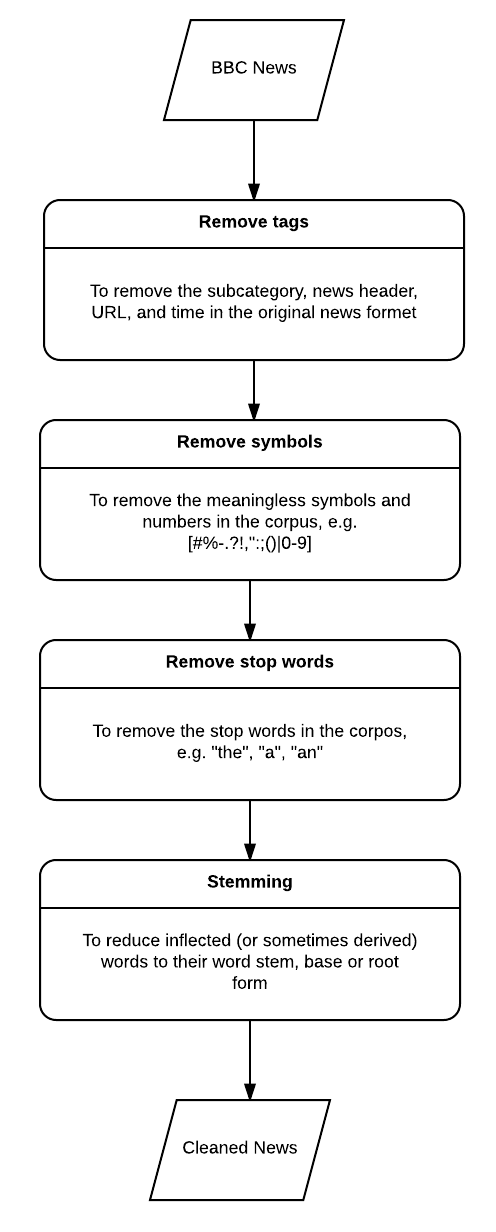
\includegraphics[width=0.5\textwidth]{figures/pipeline.png}
\caption{Preprocessing pipeline for BBC news.}
\label{fig:pipeline}
\end{figure}
\section{Baselines}
\subsection{Topic (LDA) model}

\begin{figure}[h]
\centering
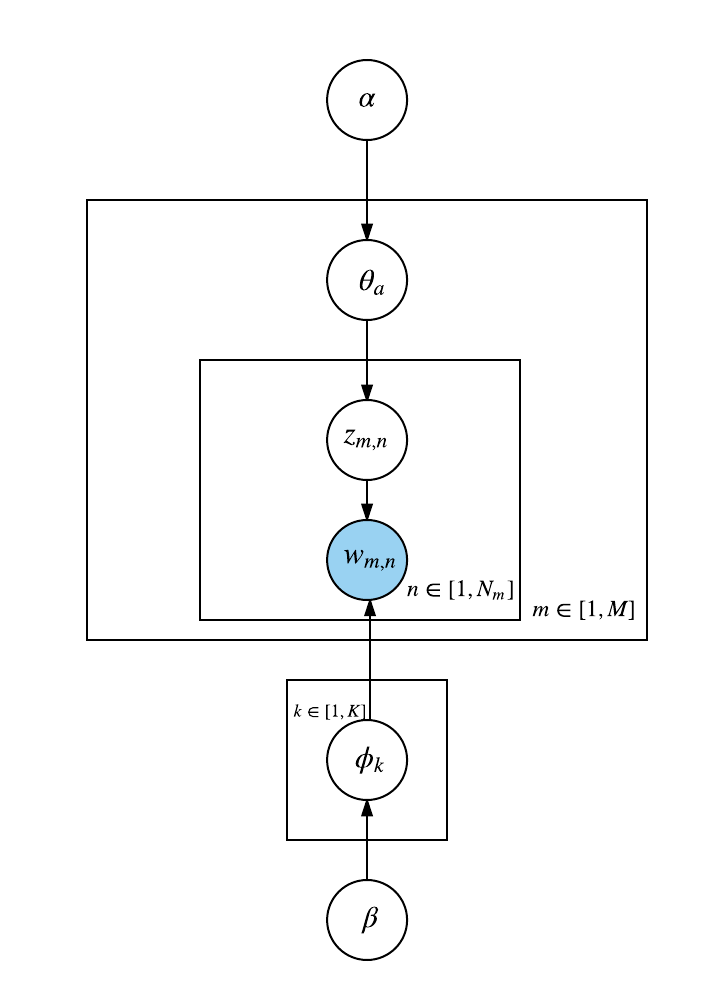
\includegraphics[width=0.6\textwidth]{figures/LDA.png}
\caption{Graphical representation of LDA topic model.}
\label{fig:atot}
\end{figure}

\subsection{Author-Topic model} \label{Author-Topic model}

 
\begin{eqnarray*} \label{eq:at}
\boldsymbol{\Theta}_a | \boldsymbol{\alpha} & \sim & \text{Dirichlet}(\boldsymbol{\alpha})\\
\boldsymbol{\Phi_{k}} | \boldsymbol{\beta} & \sim & \text{Dirichlet}(\boldsymbol{\beta})\\
z_{m,n} | \boldsymbol{\Theta_{x_{m,n}}} & \sim & \text{Multinomial}(\boldsymbol{\Theta_{x_{m,n}}})\\
w_{m,n} | \boldsymbol{\Phi_{z_{m,n}}} & \sim & \text{Multinomial}(\boldsymbol{\Phi_{z_{m,n}}})\\
x_{m,n} | A_m & \sim & \text{Multinomial}(1/A_m)\\

\end{eqnarray*}


\begin{figure}[h]
\centering
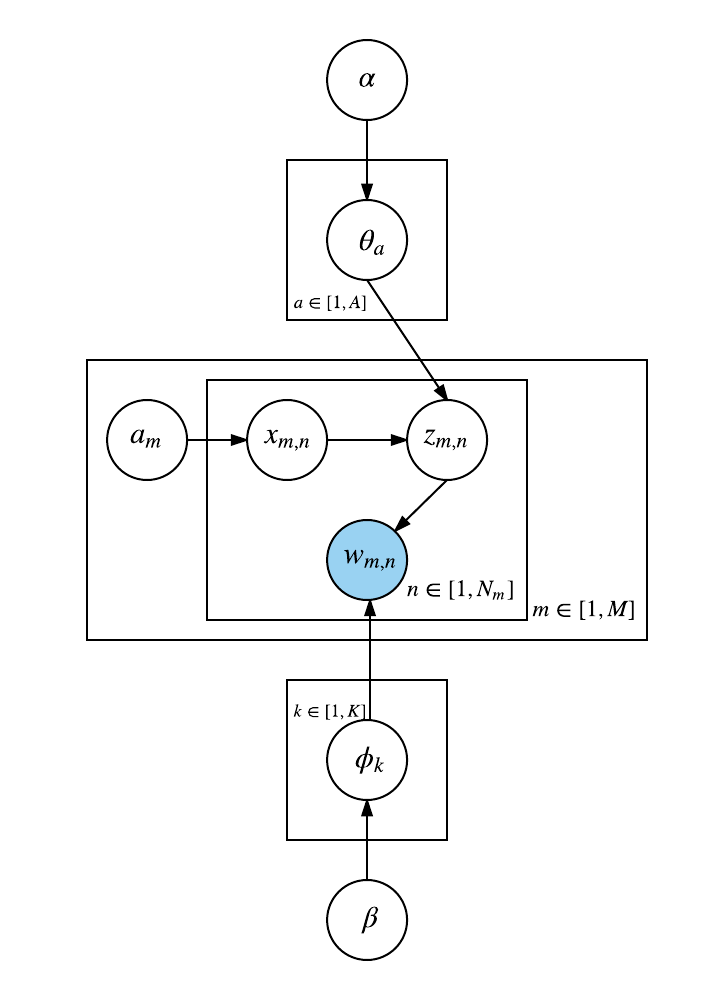
\includegraphics[width=0.6\textwidth]{figures/AT.png}
\caption{Graphical representation of Author-Topic model.}
\label{fig:atot}
\end{figure}

\subsection{Dynamic Topic model}

\begin{figure}[h]
\centering
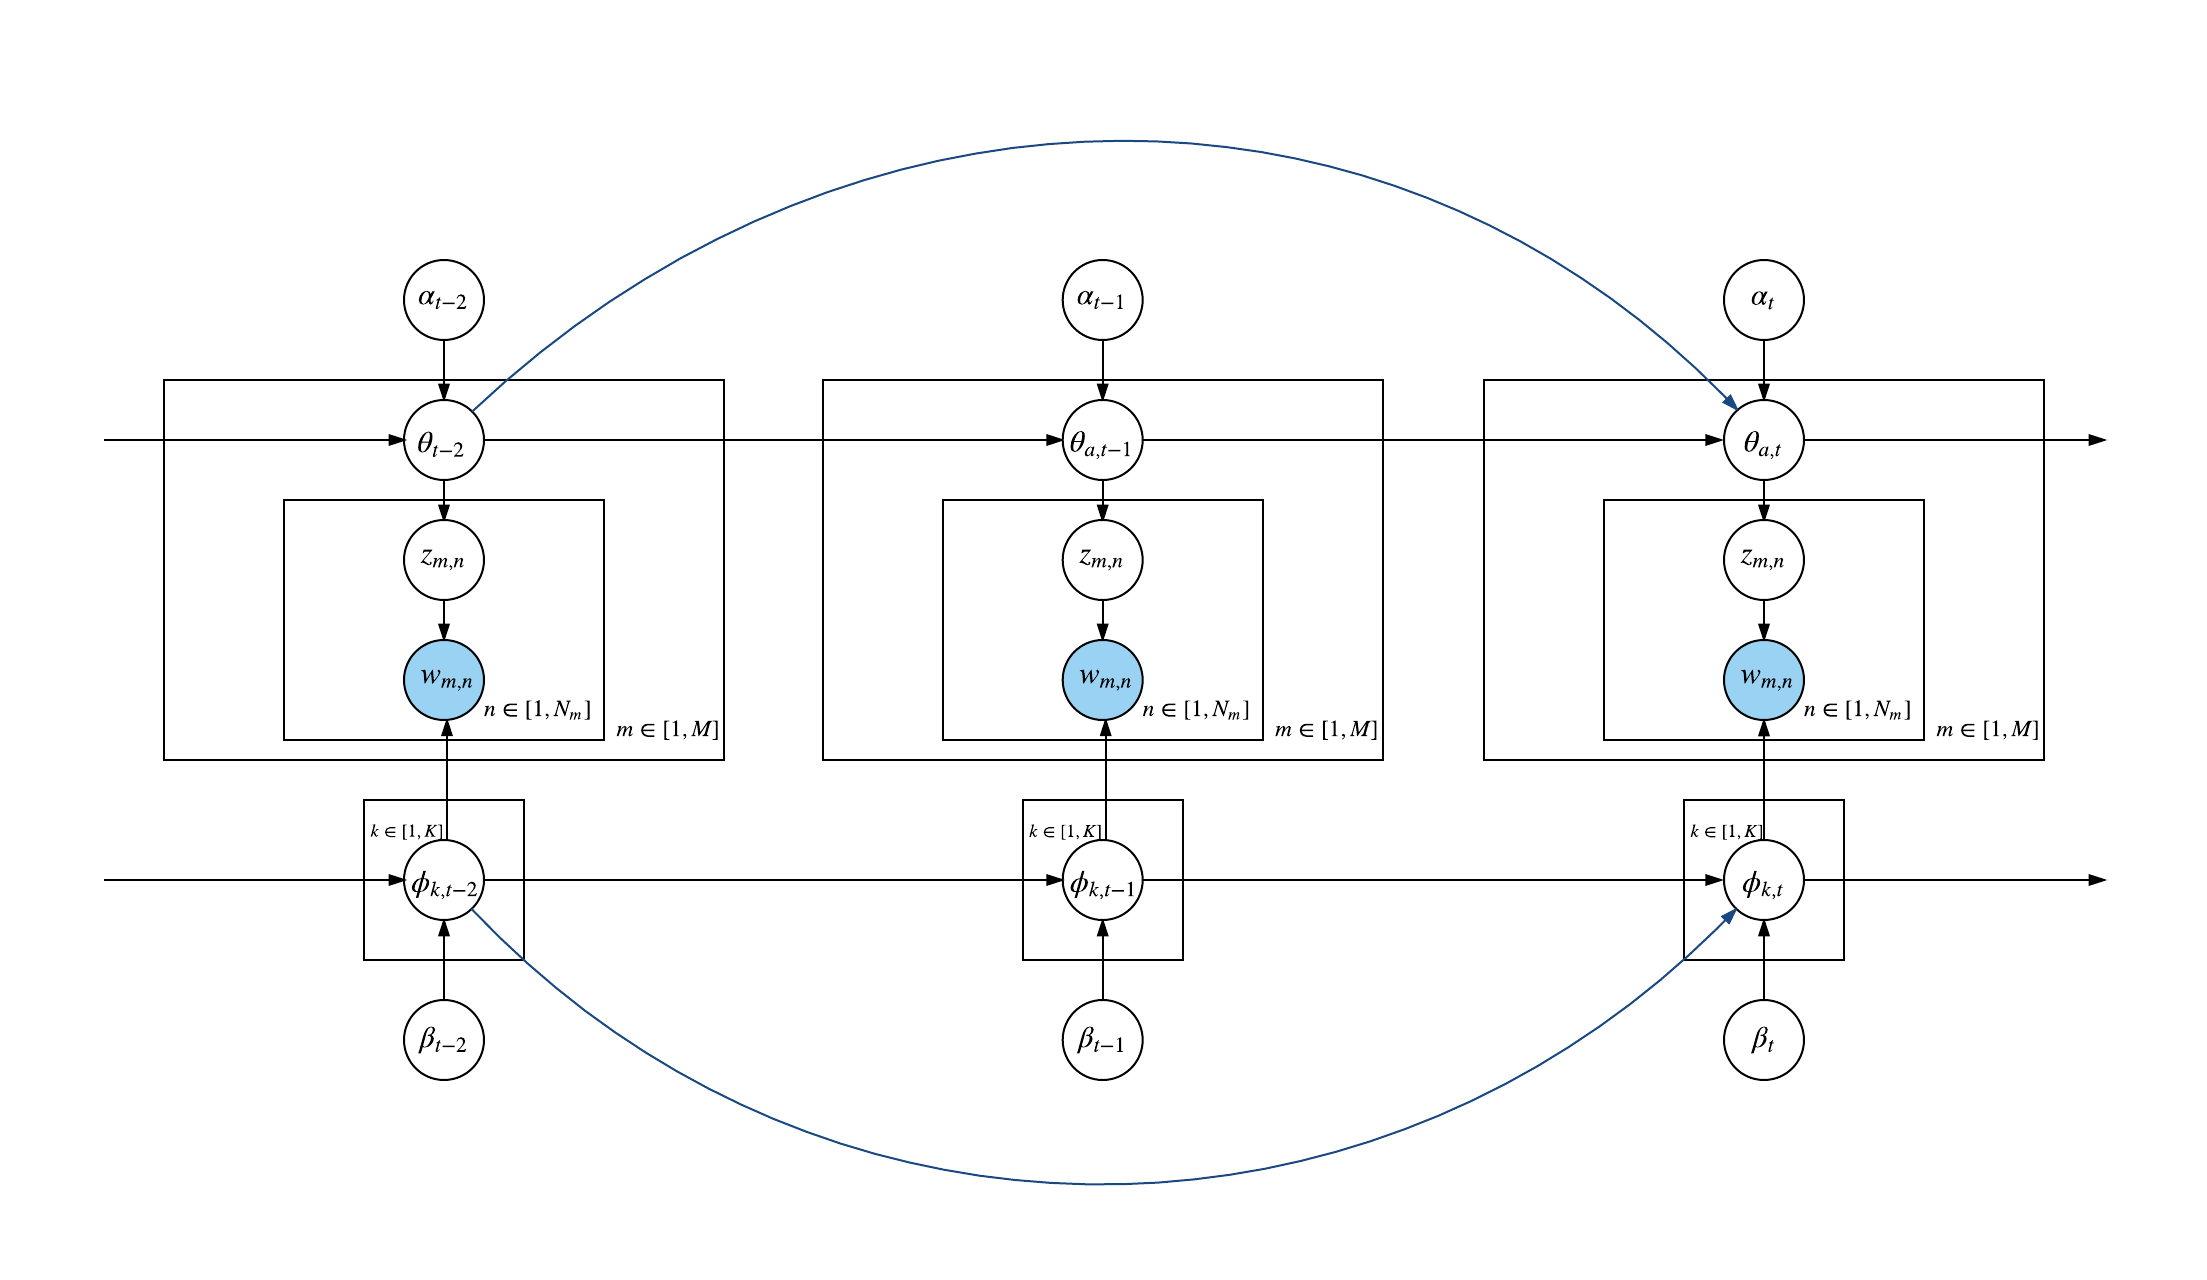
\includegraphics[width=\textwidth]{figures/TOT.png}
\caption{Graphical representation of Dynamic Topic model.}
\label{fig:atot}
\end{figure}

\section{Evaluation Metrics}
Perplexity is a common  evaluation criterion for the performance of Gibbs sampler, namely when the performance of a model trained with sampling begins to level out, which means the Markov chain reaches its convergence. In our experiment we use perpelexity to assess when the performance of our model begins to stabilize, showing how good our classification of topics and authors are.
The perplexity of a set of words is defined as the exponential of negative normalized predictive likelihood under this model, the perplexity of a news $m$
with length $N_m$ containing the set of the words $\boldsymbol{w_m}$ is conditioned on the known authors $\boldsymbol{a}$ of this news and also the time-frame $t$ since ours is a dynamic model. 

\begin{equation}\label{eq:perplexity0}
\mathcal L (\boldsymbol w)
    = \log p(\boldsymbol w | \boldsymbol a, t)
    = \sum_m \log p(\boldsymbol w_m | \boldsymbol a, t)
\end{equation}

Further, in our case we only have one author for each news, therefore if can be deducted as,
\begin{equation}\label{eq:perplexity0}
\begin{split}
\sum_m \log p(\boldsymbol w_m | \boldsymbol a, t)&=\sum_{t=1}^T\sum_{m=1}^{M_t} \log p(\boldsymbol w_m | \boldsymbol a, t)\displaybreak[1]\\
&=\sum_{m=1}^M \sum_{n=1}^{N_M}\log p(w | a_m, t)\displaybreak[1]\\
&=\sum_{m=1}^M \sum_{n=1}^{N_M}\log \sum_{k=1}^K p(w | t,k,a_m)p(k | t,a_m)\displaybreak[1]\\
\end{split}
\end{equation}

 In ~\ref{eq:perplexity0} it shows the log-likelihood of a set of news which contain the word sets $\boldsymbol{w}$ given the author of the news and the time if it is dynamic model. Likelihood of news can be used to compare models, higher likelihood implies a better model. Then the perplexity is traditionally used to measure the topic model, which is derived from \ref{eq:perplexity0}, as follows,
 \begin{equation}\label{eq:perplexity1}
 \text{perplexity}(\boldsymbol w) =
        \exp \left\{
        - \frac{\mathcal L(\boldsymbol w)}{\sum_{m=1}^M{N_m}}
        \right\}
\end{equation}
 
%\begin{equation}\label{eq:perplexity1}
%\text{Perplexity}(w_{m,n}|a_m) = exp(-\frac{\text{log} %p(w_{m,n}|a_m,M^\text{train})}{N_m})
%\end{equation}

From ~\ref{eq:perplexity1} we then drop the dependency of the hyperparameters $\alpha$ and $\beta$, we then approximate the integrals over $\boldsymbol{\theta}$ and $\boldsymbol{\phi}$ using the point estimation. By averaging over multiple samples we can finally obtain the probability $p(w_{m,n}|a_m,M^\text{train})$ as in formula ~\ref{eq:perplexity2},
\begin{equation}\label{eq:perplexity2}
p(w_{m,n}|a_m,M^\text{train}) \approx \frac{1}{S} \sum_{s=1}^{S}\prod_{n=1}^{N_m}[\frac{1}{A_m}\sum_{k}\theta_{a_m,k}\phi_{w_{m,n},k}|\boldsymbol{x^s},\boldsymbol{z^s},M^\text{train},\alpha,\beta]
\end{equation}

in which $A_m = 1$. 
\chapter{Results and Analysis}
\label{chapterlabel5}

\section{Performance Comparison between Dynamic Author-topic model and LDA model}
\section{Performance Comparison between Dynamic Author-topic model and Author-topic Model}

Author-topic model: $\alpha = 0.5$, $\beta = 0.1$, $\text{Author Number} = 9$
Dynamic Author-topic model: $\alpha = 0.1$, $\beta = 0.1$, $\text{Author Number} = 9$

\subsection{Perplexity}
\subsection{Author Distribution}
\subsection{Topic Distribution}
\subsection{Illustration of author-topic-words}

\section{Performance Comparison between Dynamic Author-topic model and Dynamic Topic Model}
\section{Comprehensive comparison}
\section{Performance with different time slices}
\section{Performance with different topic number}

% This just dumps some pseudolatin in so you can see some text in place.
\blindtext

\chapter{Conclusions}
\label{chapterlabel6}

\section{Summary of the thesis}
\section{Future work}

% This just dumps some pseudolatin in so you can see some text in place.
\blindtext

\addcontentsline{toc}{chapter}{Appendices}

% The \appendix command resets the chapter counter, and changes the chapter numbering scheme to capital letters.
%\chapter{Appendices}
\appendix
\chapter{Code}
\label{appendixlabel1}
(stuff)

%\chapter{Another Appendix About Things}
%\label{appendixlabel2}
%(things)

%\chapter{Colophon}
%\label{appendixlabel3}
%\textit{This is a description of the tools you used to make your thesis. It helps people make future documents, reminds you, and looks good.}

%\textit{(example)} This document was set in the Times Roman typeface using \LaTeX\ and Bib\TeX , composed with a text editor. 
 % description of document, e.g. type faces, TeX used, TeXmaker, packages and things used for figures. Like a computational details section.
% e.g. http://tex.stackexchange.com/questions/63468/what-is-best-way-to-mention-that-a-document-has-been-typeset-with-tex#63503

% Side note:
%http://tex.stackexchange.com/questions/1319/showcase-of-beautiful-typography-done-in-tex-friends 
% You could separate these out into different files if you have
%  particularly large appendices.

% This line manually adds the Bibliography to the table of contents.
% The fact that \include is the last thing before this ensures that it
% is on a clear page, and adding it like this means that it doesn't
% get a chapter or appendix number.
\addcontentsline{toc}{chapter}{Bibliography}

% Actually generates your bibliography.
\bibliography{example}

% All done. \o/
\end{document}
